\documentclass[a4paper]{article}

% CJK support: prefer ctex, fallback to XeTeX native line breaking
\IfFileExists{ctex.sty}{
  \usepackage[fontset=fandol]{ctex}
}{
  \usepackage{fontspec}
  \XeTeXlinebreaklocale "zh"
  \XeTeXlinebreakskip = 0pt plus 1pt
  \IfFontExistsTF{Songti SC}{\setmainfont{Songti SC}}{%
    \IfFontExistsTF{Noto Serif CJK SC}{\setmainfont{Noto Serif CJK SC}}{}%
  }
  \IfFontExistsTF{Heiti SC}{\setsansfont{Heiti SC}}{%
    \IfFontExistsTF{Noto Sans CJK SC}{\setsansfont{Noto Sans CJK SC}}{}%
  }
}

% Basic packages
\usepackage{amsmath, amssymb}
\usepackage{graphicx}
\usepackage[margin=2.5cm]{geometry}
\emergencystretch=3em
\usepackage[most]{tcolorbox}
\usepackage{etoolbox}
\usepackage{listings}
\usepackage{hyperref}
\hypersetup{hidelinks,pdftitle={如何真正信任你的编码智能体：闭环验证、技能评测与面向智能体友好的架构重构},pdfauthor={Lauren Tan (@poteto)}}
\usepackage{booktabs}
\usepackage{array}
\usepackage{subcaption}
\usepackage{float}

% ===== Highlight boxes =====
\newtcolorbox{knowledgebox}[1]{
    enhanced, colback=black!2!white, colframe=black!65, colbacktitle=black!65,
    coltitle=white, fonttitle=\bfseries, title=#1, attach boxed title to top left={yshift=-2mm, xshift=2mm},
    boxrule=1pt, sharp corners
}

\newtcolorbox{importantbox}[1]{
    enhanced, colback=red!3!white, colframe=red!45!black, colbacktitle=red!45!black,
    coltitle=white, fonttitle=\bfseries, title=#1, sharp corners
}

\newtcolorbox{warningbox}[1]{
    enhanced, colback=red!5!white, colframe=red!75!black, colbacktitle=red!75!black,
    coltitle=white, fonttitle=\bfseries, title=#1, sharp corners
}

\newtcolorbox{practicebox}[1]{
    enhanced, colback=black!3!white, colframe=black!75, colbacktitle=black!75,
    coltitle=white, fonttitle=\bfseries, title=#1, sharp corners
}

% ===== Code listings =====
\lstset{
    basicstyle=\ttfamily\small,
    keywordstyle=\color{blue},
    stringstyle=\color{red!60!black},
    commentstyle=\color{green!60!black},
    breaklines=true,
    frame=single,
    numbers=left,
    numberstyle=\tiny\color{gray},
    captionpos=b,
    extendedchars=false
}

% ===== Figure provenance and unit macros =====
\newcommand{\vtag}{\protect\footnotemark}
\newcommand{\srcnote}[1]{\footnotetext{视频画面时间区间：#1。若为裁剪图，时间区间仍对应原视频画面。}}

% ===== Front-page metadata =====
\newcommand{\notetitle}{如何真正信任你的编码智能体}
\newcommand{\notesubtitle}{闭环验证（control-glass）、技能单元测试（pstack）、云端复现智能体（Benny）与面向智能体友好的强约束架构（Dune）}
\newcommand{\noteauthors}{Lauren Tan (@poteto，Cursor / Anysphere 软件工程师) 主讲 · lecture-to-notes 整理}
\newcommand{\notedate}{2026 年 10 月 27 日}
\newcommand{\videochannel}{Lauren Tan 主讲 / Colin 主持 / @tsukiema\_ 上传}
\newcommand{\videopublishdate}{20261025}
\newcommand{\videoduration}{54 分 07 秒}
\newcommand{\videourl}{https://x.com/tsukiema_/status/2114360674432303569/video/1}
\newcommand{\videocoverpath}{cover.jpg}

\begin{document}

% ===== Title page =====
\begin{titlepage}
\centering
{\Large 课程笔记\par}
\vspace{1.2cm}
{\huge\bfseries \notetitle\par}
\ifdefempty{\notesubtitle}{}{
\vspace{0.3cm}
{\large \notesubtitle\par}
}
\vspace{0.5cm}
{\large \noteauthors\par}
\vspace{0.3cm}
{\large \notedate\par}
\vspace{1.0cm}

\ifdefempty{\videocoverpath}{
{\small 请在生成笔记时填入视频封面图的本地路径。\par}
}{
\includegraphics[width=0.82\textwidth,height=0.40\textheight,keepaspectratio]{\videocoverpath}\par
}

\vfill
\begin{tcolorbox}[width=0.9\textwidth, colback=black!2!white, colframe=black!60, sharp corners]
\textbf{视频作者/频道}：\videochannel\par
\textbf{发布日期}：\videopublishdate\par
\textbf{视频时长}：\videoduration\par
\textbf{视频链接}：\ifdefempty{\videourl}{待填写}{\url{\videourl}}\par
\end{tcolorbox}
\end{titlepage}

% ===== Executive Summary =====
\begin{importantbox}{核心主旨与视频来源双向考证说明}
本讲义整理自资深软件工程师 \textbf{Lauren Tan}（GitHub ID：\texttt{poteto}，前 Meta 工程师）关于\textbf{“如何建立对编码智能体（Coding Agents）的工程级信任，并在 5 个月内单人高质量合并 3,000+ 个 PR”}的深度技术分享及炉边访谈。

\textbf{视频来源考证（Provenance Note）}：本视频由 X 账号 \texttt{@tsukiema\_} 转播发布。通过对全分辨率共享屏幕画面的逐帧源码级核验可以确认，演讲的真实工程底座是 \textbf{Cursor（Anysphere）}：屏幕画面中清晰展示了 Cursor 内部仓库路径 \texttt{.cursor/skills/client/control-glass/SKILL.md}、安全与构建评审组 \texttt{anysphere/security-reviewers} 与 \texttt{anysphere/build-reviewers}、Agents Window 内部代号 \textbf{\texttt{Glass}}、云端值班频道 \texttt{\#glass-oncall-assistant} 以及新一代多智能体编排桌面端仓库 \texttt{sand/dune} 与 \texttt{sand/src}。转播者在视频左上角叠加了伪造铭牌（甚至将 \texttt{SpaceXAI} 拼错为 \texttt{SpaxeXAI}），并在音轨中将主讲人口述的 \texttt{Cursor}、\texttt{Sand}、\texttt{Claude 4.6} 局部拼接替换为了 \texttt{SpaceXAI}、\texttt{GrokBot}、\texttt{Grok 4.6}。为保证技术文献的绝对真实性与可检索性，本讲义以屏幕展示的\textbf{真实工程命名（Cursor / Glass / Sand / Dune / pstack）}为主线，同时在对应处标注音轨中的替换词，帮助读者还原 100\% 准确的工程全貌。
\end{importantbox}

\tableofcontents
\newpage

% ============================================================================
\section{从“AI 结对编程”到跨越智能体信任曲线}
% ============================================================================

\subsection{抵御外包思考与“Vibe Coding”生产力泡沫（00:00--02:30）}

在 AI 编码工具席卷软件行业的当下，几乎每一位软件工程师都感受到一种无形的同辈压力：仿佛如果不把 AI 塞进每一个工作流、不在社交媒体上炫耀“我这周用 AI 生成并合并了 100 个 PR”，自己就会被时代淘汰。然而，曾在 Meta 等大型科技公司深耕多年、对软件架构与代码质量有着极高标准（Opinionated）的资深工程师们，在真正把编码智能体引入核心生产环境时，往往会遭遇强烈的挫败感。

\begin{figure}[H]
  \centering
  
\includegraphics[width=0.84\textwidth]{figures/fig_01_speaker_intro.png}
  \caption{主讲人 Lauren Tan（\texttt{@poteto}）开场探讨工程师在高速交付压力与工程质量标准之间的核心矛盾\vtag}
\end{figure}
\srcnote{00:00:30--00:00:45}

Lauren Tan 在开场便指出，这种挫败感的根源在于混淆了\textbf{“AI 结对编程（Pair Programming）”}与\textbf{“把思考外包给 AI（Outsourcing Your Thinking）”}：
\begin{itemize}
  \item \textbf{Vibe Coding 的认知负债}：如果一个人声称自己一周合并了 100 个 PR，但对其中的实现逻辑、边界条件与系统副作用一无所知，那并不是工程生产力的提升，而是在以指数级速度向代码库倾倒技术债。
  \item \textbf{“第 100 次盲目自信”的幻觉疲劳}：在复杂系统排障中，未经约束的编码智能体极易陷入盲目猜测（Winging it / Guessing）。许多工程师都有过类似的崩溃体验：智能体连续第 100 次在对话框里信誓旦旦地宣布“我已经找到了确凿的元凶（Smoking Gun）！”，结果人类工程师花半小时一查，发现它连调用链都没看懂，完全是在胡说八道。
  \item \textbf{从写代码转移到审代码的隐性耗时}：许多工程师以为用 AI 写代码省下了敲键盘的时间，但实际上却把更多的时间、精力和情绪消耗在了痛苦的人工代码审查（Code Review）、手动拉起分支验证以及替智能体收拾残局上。
\end{itemize}

\subsection{工程管理类比与智能体信任曲线（02:30--04:30）}

为什么大多数工程师无法同时驾驭超过 3 个编码智能体？Lauren 借用了她过去担任\textbf{工程经理（Engineering Manager, EM）}和团队技术负责人（Tech Lead）的经验给出了精辟的类比：当你使用编码智能体时，你的角色本质上已经从单兵作战的程序员转变为\textbf{管理一支智能体工程团队的经理}。

在人类工程团队管理中，如果你对下属的能力或工作方式缺乏信任，你的本能反应必然是\textbf{微观管理（Micromanagement）}——你会紧盯他们写的每一行代码、每一个技术决策，不敢放手让他们独立负责模块。这种微观管理模式在面对智能体时表现为完全相同的瓶颈：

\begin{figure}[H]
  \centering
  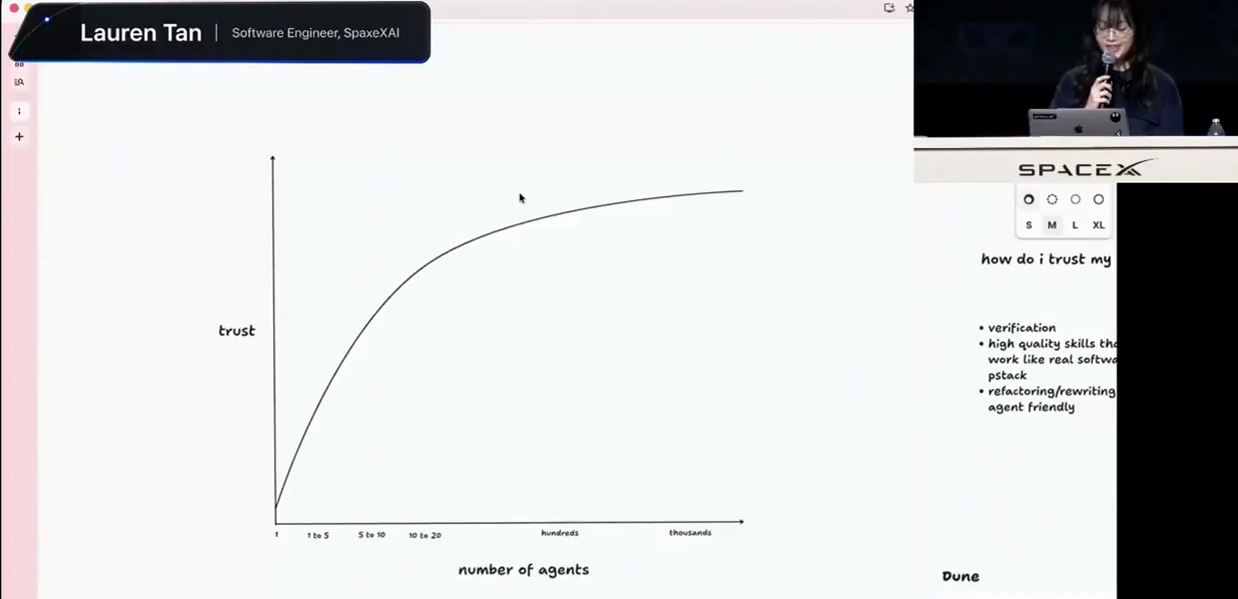
\includegraphics[width=0.88\textwidth]{figures/fig_02_trust_curve.png}
  \caption{智能体信任曲线（The Agent Trust Curve）：横轴为可并行调度的智能体数量（从 1、1--5、5--10、10--20 到数百乃至数千），纵轴为工程师对智能体系统的信任度（\texttt{trust}）\vtag}
\end{figure}
\srcnote{00:01:45--00:02:00}

如图 2 所示，工程师能够有效并行调度的智能体数量 $N_{\text{agents}}$，严格受限于其对智能体闭环体系的信任度 $\mathcal{T} \in [0, 1)$ 与单智能体所需的人工盯防介入率 $(1 - \mathcal{T})$。设人类工程师的总注意力带宽上限为 $B_{\text{human}}$，每次人工审查与纠偏的平均认知开销为 $c_{\text{review}}$，则可维持的并行智能体规模满足如下关系：
\begin{equation}
  N_{\text{agents}}(\mathcal{T}) \;\propto\; \frac{B_{\text{human}}}{c_{\text{review}} \cdot (1 - \mathcal{T}) + c_{\text{orchestrate}}}
\end{equation}
从式 (1) 可以清晰地看出两个演化阶段：
\begin{enumerate}
  \item \textbf{低信任微观管理区（$N_{\text{agents}} \in [1, 5]$）}：当信任度 $\mathcal{T}$ 较低时，$(1 - \mathcal{T})$ 居高不下。人类必须像保姆一样紧盯智能体的每一次工具调用（Tool Call）和每一行 Diff。此时并行的智能体哪怕增加到 3--5 个，人类的注意力带宽 $B_{\text{human}}$ 就会瞬间饱和，沦为整个系统的单线程吞吐瓶颈。
  \item \textbf{高信任边际扩展区（$N_{\text{agents}} \in [10, 10^3]$）}：只有当工程体系建立起严密的自动验证与架构护栏，使信任度 $\mathcal{T} \to 1$（即人工盯防成本趋近于零，仅保留极低的编排巡检成本 $c_{\text{orchestrate}}$）时，曲线才会越过拐点，解锁同时调度 10--20 个本地/工作树智能体、乃至在云端并发运行数百上千个智能体的规模化能力。
\end{enumerate}

\subsection{5 个月合并 3,000+ 个 PR 的产能跃迁与三大工程支柱（04:30--06:30）}

为了证明“高信任度智能体工程体系”并非纸上谈兵，Lauren 展示了她加入 Cursor（Anysphere）短短 5 个月以来的真实 GitHub 贡献曲线：

\begin{figure}[H]
  \centering
  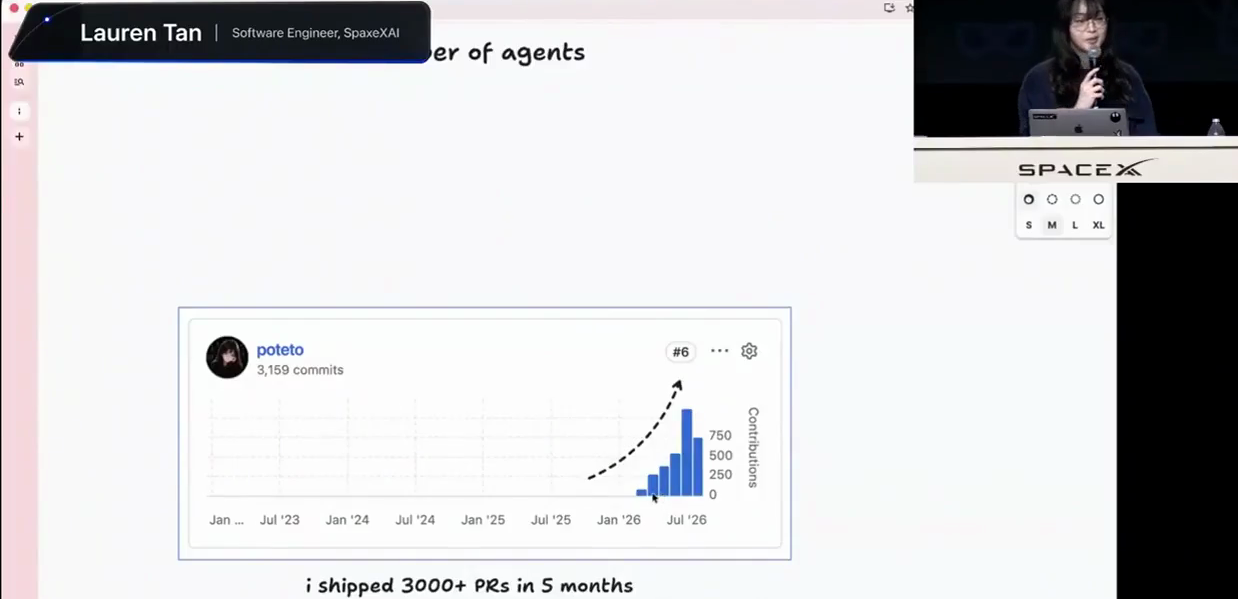
\includegraphics[width=0.88\textwidth]{figures/fig_03_poteto_3000_prs.png}
  \caption{Lauren Tan（GitHub ID：\texttt{poteto}）在 5 个月内合并 3,000+ 个 PR（累计 3,159 commits，位列内部贡献榜第 6 名）的指数级产能跃迁曲线\vtag}
\end{figure}
\srcnote{00:04:45--00:05:00}

图 3 中的蓝色柱状图清晰记录了她跨越信任曲线的全过程：
\begin{itemize}
  \item \textbf{第 1 个月（冷启动期）}：刚加入公司时，她和普通工程师一样，一边熟悉庞大的代码库，一边尝试用常规方式驱动智能体，当月 PR 合并量十分平缓。
  \item \textbf{第 2--4 个月（基建期）}：她将重心转向解决“为什么我不敢信任智能体”的根本原因，陆续构建了客户端自动化验证工具、团队共享技能库以及强约束架构。贡献量呈现陡峭的指数级攀升。
  \item \textbf{第 5 个月（爆发期）}：在演讲前的上个月，她单月合并了约 1,000 个 PR；而在演讲当月的前 12 天里，她已经合并了将近 800 个 PR（按此速率折算单月可达 2,000 个 PR），5 个月累计交付 \textbf{3,000+ 个 PR}（共 3,159 commits）。
  \item \textbf{“睡后自动合并”与事后主干巡检}：Lauren 分享道，就在演讲当天早上她醒来时，后台运行的智能体已经在夜间自动通过了所有端到端验证与 CI 门禁，将大约 \textbf{20 个 PR 自动合并（Auto-merged）}进了 \texttt{main} 主干分支。她早上的工作不再是逐行审批未合并的 PR，而是在 \texttt{main} 分支上做轻量级的事后巡检（Post-merge Spot Check），确认整体行为符合预期；即便偶有瑕疵，由于每个 PR 都极其短小原子化，随时可以一键回滚或追加修正。
\end{itemize}

\begin{figure}[H]
  \centering
  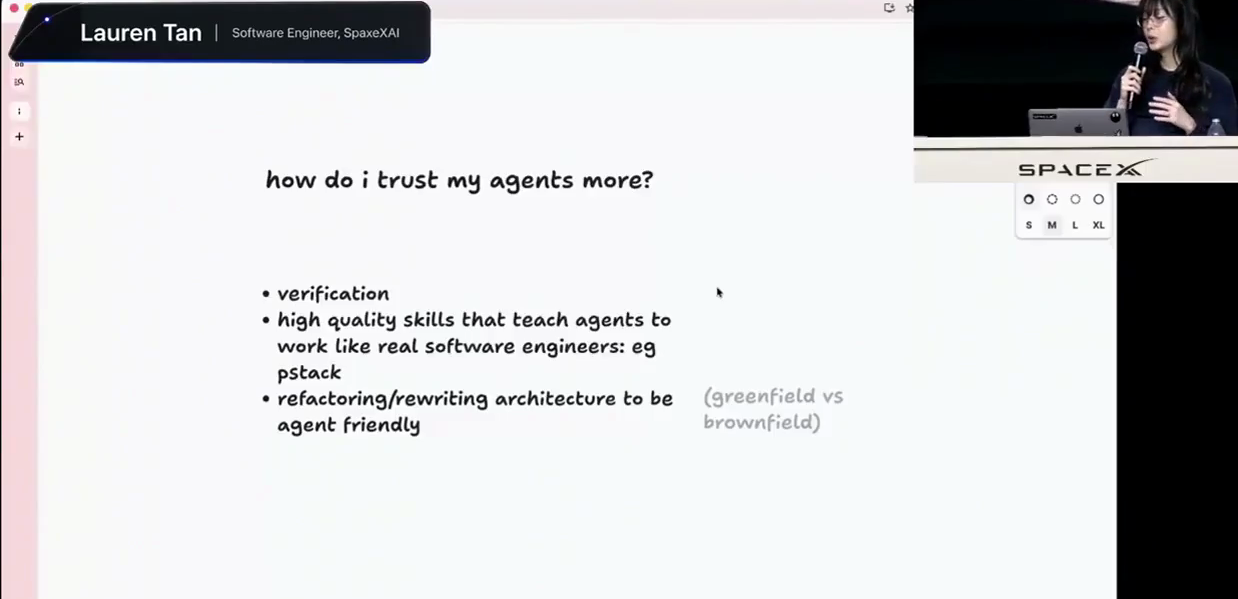
\includegraphics[width=0.88\textwidth]{figures/fig_04_three_pillars.png}
  \caption{回答“我该如何更加信任我的智能体（\texttt{how do i trust my agents more?}）”的三大工程支柱总览\vtag}
\end{figure}
\srcnote{00:06:00--00:06:15}

那么，究竟如何把信任度 $\mathcal{T}$ 推向这根曲线的顶端？如图 4 所示，Lauren 将其总结为三大核心工程支柱：
\begin{enumerate}
  \item \textbf{支柱一：闭环验证（Verification）}——赋予智能体像人类工程师一样启动真实应用、点击交互、采集性能剖析并自行验证代码改动的能力（代表作：内部技能 \texttt{control-glass} 与功能导航地图 \texttt{feature-map.md}）。
  \item \textbf{支柱二：高质量工程技能库与技能评测（High-Quality Skills \& Evals）}——将资深软件工程师的排障方法论沉淀为可复用的技能包（代表作：开源插件 \texttt{pstack}），并为其构建防作弊的“技能单元测试”（\texttt{eval-playbook}）。
  \item \textbf{支柱三：面向智能体友好的架构重构（Agent-Friendly Architecture）}——针对从零演化的新项目（Greenfield），顺应智能体的局部上下文贪婪本能，设计出“最短路径即正确路径”的强约束框架（代表作：\texttt{Dune} 架构及其五层防御金字塔）。
\end{enumerate}

\subsection{本章小结}

本章剖析了 AI 时代软件工程师面临的核心困境：如果缺乏系统性的信任机制，使用 AI 只会让人陷入紧盯 1--3 个智能体的微观管理与代码审查疲劳。通过引入工程管理视角与智能体信任曲线（式 (1)），我们看到唯有通过闭环验证、高质量工程技能与强约束架构三大支柱将人工盯防率降至接近零，才能实现单人 5 个月高质量交付 3,000+ 个 PR 的生产力飞跃。

\clearpage
% ============================================================================
\section{第一支柱：闭环验证（Verification）——\texttt{control-glass} 与 \texttt{feature-map.md}}
% ============================================================================

\subsection{砍掉“人肉验证瓶颈”：从手动抓火焰图到 \texttt{control-glass}（06:00--08:00）}

在与编码智能体协作的所有工具箱中，Lauren 认为\textbf{最重要、排序第一的能力永远是闭环验证（Verification）}。这里的验证绝不仅仅指跑通单元测试（Unit Tests）或类型检查（Typecheck）——因为单元测试往往在 Mock 环境中运行，完全可能出现“测试全部变绿，但真实桌面端界面点击没反应或严重卡顿”的情况。真正的闭环验证，是让智能体能够在\textbf{无需人类介入的情况下，自己把真实软件跑起来并完成端到端检验}。

Lauren 回忆了她刚加入 Cursor 第一周时的亲身经历：当时团队正在全力冲刺发布全新的多智能体窗口界面——\textbf{Agents Window}（内部研发代号为 \textbf{\texttt{Glass}}，这是一个基于 Electron 与 React 构建的复杂桌面应用程序）。为了排查界面卡顿与渲染性能瓶颈，她最初的工作流是：
\begin{enumerate}
  \item 自己手动编译并打开 Electron 开发版客户端；
  \item 手动打开 Chrome DevTools 的 Performance 面板，点击录制，在界面上复现卡顿操作；
  \item 停下录制，找到异常的火焰图（Flame Graph）或控制台报错，手动截图并复制堆栈信息；
  \item 把截图和日志粘贴回对话框喂给智能体，等智能体改完代码后，自己再手动重复一遍上述流程。
\end{enumerate}

她很快意识到：\textbf{在这个反馈回路中，人类自己成了最慢的“人肉验证器瓶颈（Human as the Verifier Bottleneck）”}。只要验证还需要人类亲手点鼠标、截屏幕，你就永远不可能同时并行跑 10 个智能体。于是，她动手构建了内部验证技能——\textbf{\texttt{control-glass}}。

\begin{figure}[H]
  \centering
  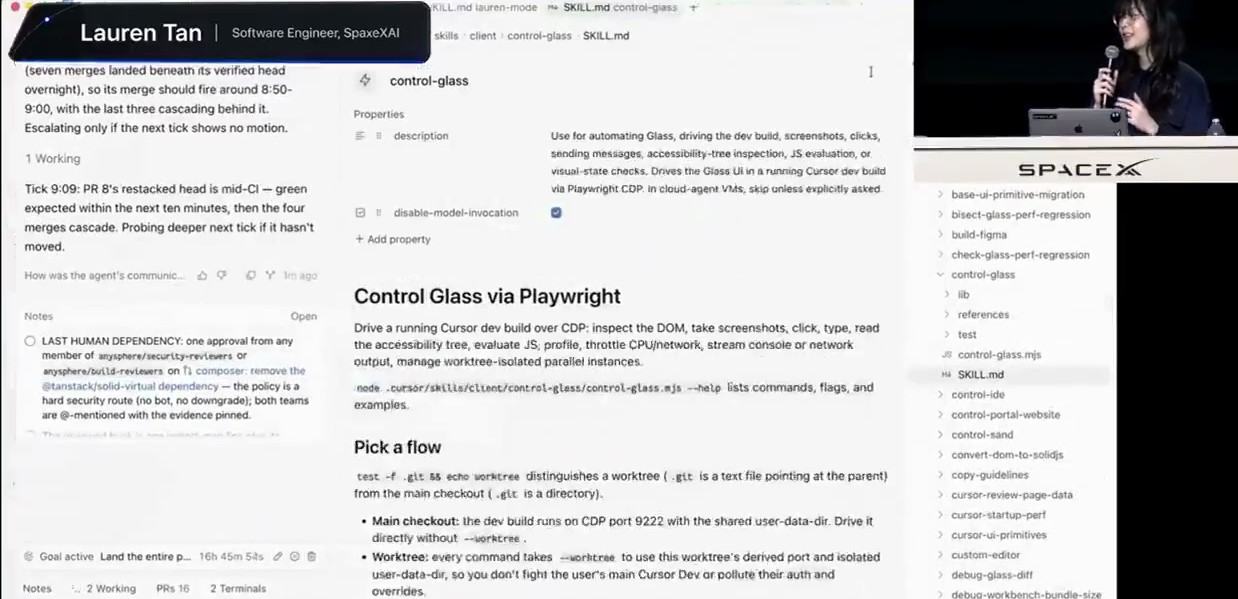
\includegraphics[width=0.92\textwidth]{figures/fig_05_control_glass_skill.png}
  \caption{Cursor 内部 \texttt{.cursor/skills/client/control-glass/SKILL.md} 技能文档总览。注意左侧边栏展示了正在自动推进的 16 个 PR 任务栈与安全评审组 \texttt{anysphere/security-reviewers} 门禁状态\vtag}
\end{figure}
\srcnote{00:07:00--00:07:15}

如图 5 所示，\texttt{control-glass}（全称 \texttt{Control Glass via Playwright}）是一个通过 \textbf{Playwright} 连接 \textbf{Chrome DevTools Protocol（CDP）}来直接驱动运行态 Cursor 开发版客户端（Dev Build）的自动化技能。智能体只需调用一行命令：
\begin{lstlisting}[language=bash]
node .cursor/skills/client/control-glass/control-glass.mjs --help
\end{lstlisting}
即可获取完整的客户端控制能力，包括：检查实时 DOM 结构、读取无障碍树（Accessibility Tree）、截取局部或全屏画面、模拟真实鼠标点击与键盘按键输入、在渲染进程执行任意 JavaScript 表达式（\texttt{eval}）、采集 CPU 火焰图与网络性能剖析（Profile）、模拟 CPU/网络限速（Throttle），以及实时流式读取控制台（Console）与网络请求日志。

\begin{knowledgebox}{图 5 左侧边栏解析：一窥自动运转的 PR 级联流水线}
仔细观察图 5 左侧的 Cursor Notes 面板，可以看到 Lauren 后台正在运行的自动化目标（\texttt{Goal active: Land the entire p... 16h 45m}，共管理 \texttt{PRs 16}）：
\begin{itemize}
  \item 智能体自动汇报进度：\texttt{Tick 9:09: PR 8's restacked head is mid-CI --- green expected within the next ten minutes, then the four merges cascade.}（PR 8 重新变基后的头部正在跑 CI，预计 10 分钟内变绿，随后 4 个下游 PR 将自动级联合并）。
  \item 唯一需要人类介入的硬性安全门禁被清晰置顶高亮：\texttt{LAST HUMAN DEPENDENCY: one approval from any member of anysphere/security-reviewers or anysphere/build-reviewers on composer: remove the @tanstack/solid-virtual dependency --- the policy is a hard security route (no bot, no downgrade)}.
\end{itemize}
这直观展示了当验证与 CI 完全自动化后，人类工程师只需在涉及硬性安全路由（Security Route）的极少数节点点击一次审批即可。
\end{knowledgebox}

\subsection{\texttt{Pick a flow} 与 Git Worktree 隔离：十几个智能体并行驱动客户端（08:00--10:00）}

当你在本地开发机上只运行 1 个智能体时，让它通过默认 CDP 端口 \texttt{9222} 连接你正在使用的开发版客户端似乎没有问题。但一旦你试图使用 \textbf{Git Worktree} 同时拉起 5--10 个智能体并行开发不同特性或修复不同 Bug 时，灾难就会发生：所有智能体都会去争抢端口 \texttt{9222}，在同一个窗口里乱点鼠标、互相覆盖状态，甚至把你主开发窗口的登录态（Auth）和本地配置彻底搞乱！

为了彻底解决多智能体并发冲突，\texttt{control-glass} 设计了极其严密的 \textbf{\texttt{Pick a flow}} 环境分流与 Worktree 隔离机制：

\begin{figure}[H]
  \centering
  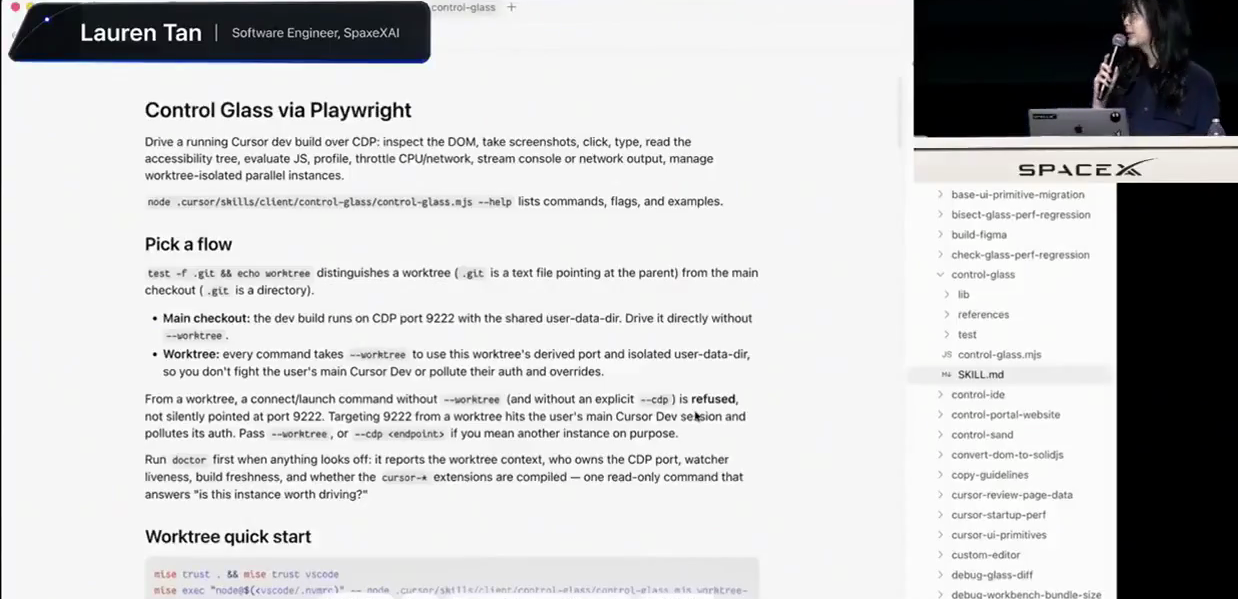
\includegraphics[width=0.92\textwidth]{figures/fig_06_pick_a_flow.png}
  \caption{\texttt{control-glass} 的 \texttt{Pick a flow} 环境分流规范：严格区分主检出目录（端口 \texttt{9222}）与 Git Worktree 独立环境（强制要求 \texttt{--worktree} 标志）\vtag}
\end{figure}
\srcnote{00:08:00--00:08:15}

如图 6 所示，\texttt{control-glass} 首先通过一行极简的 Shell 探针判断当前智能体所处的工作目录类型：
\begin{lstlisting}[language=bash]
test -f .git && echo worktree
\end{lstlisting}
在 Git 的底层实现中，主检出仓库（Main Checkout）下的 \texttt{.git} 是一个\textbf{目录（Directory）}；而在通过 \texttt{git worktree add} 创建的工作树下，\texttt{.git} 是一个指向父仓库的\textbf{纯文本文件（Text File）}。基于这一确定性判据，\texttt{control-glass} 强制执行两条分流铁律：
\begin{enumerate}
  \item \textbf{Main checkout（主检出目录）}：开发构建运行在默认 CDP 端口 \texttt{9222} 并使用共享的 \texttt{user-data-dir}，仅在主目录操作时可直接驱动（无需传 \texttt{--worktree}）。
  \item \textbf{Worktree（独立工作树）}：每一条命令都必须携带 \texttt{--worktree} 标志，工具会根据当前 Worktree 路径确定性地派生出一个\textbf{专属的独立 CDP 端口}和\textbf{物理隔离的 \texttt{user-data-dir}}。更关键的是，如果智能体身处 Worktree 却忘了传 \texttt{--worktree}（且未显式指定 \texttt{--cdp}），\texttt{control-glass} 会\textbf{直接拒绝执行并报错（Refused）}，绝不静默回退到端口 \texttt{9222}，从而从机制上杜绝了智能体误闯人类主开发窗口或污染登录态的可能。
\end{enumerate}

\begin{figure}[H]
  \centering
  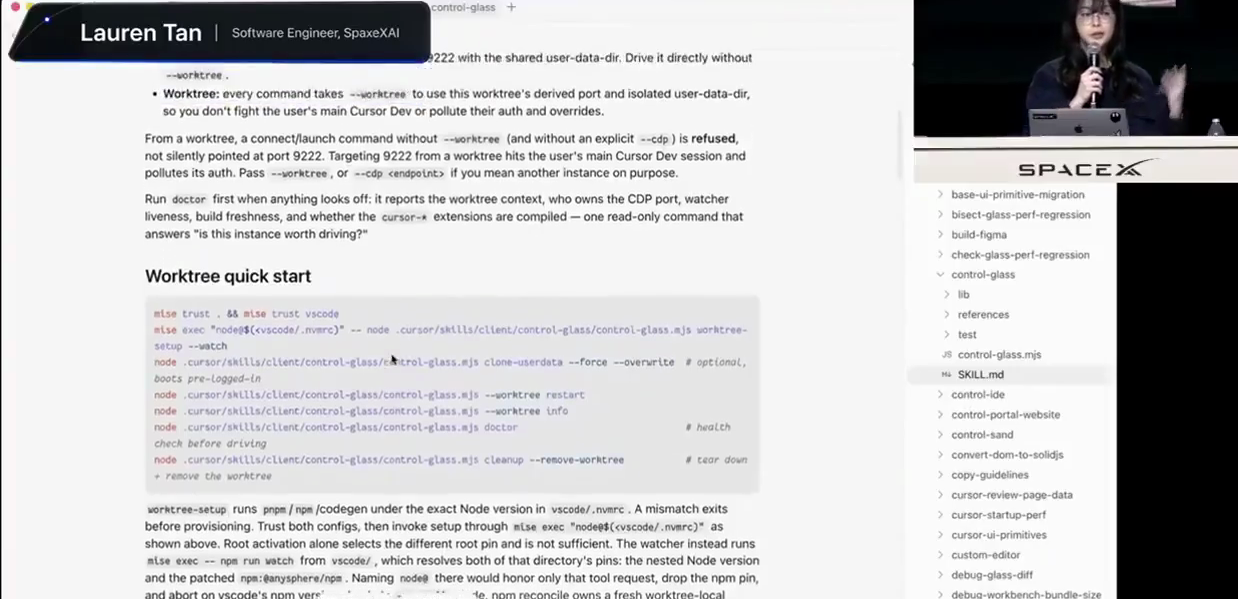
\includegraphics[width=0.92\textwidth]{figures/fig_07_worktree_quickstart.png}
  \caption{\texttt{Worktree quick start} 完整生命周期脚本：集成 \texttt{mise} 精确 Node 版本对齐、\texttt{clone-userdata} 免登录态克隆、\texttt{doctor} 健康探针与 \texttt{cleanup} 销毁回收\vtag}
\end{figure}
\srcnote{00:09:30--00:09:45}

紧接着，图 7 展示了智能体在独立 Worktree 中拉起并验证全新客户端实例的标准 6 步流水线（\texttt{Worktree quick start}）：
\begin{lstlisting}[language=bash]
mise trust . && mise trust vscode
mise exec "node@$(<vscode/.nvmrc)" -- node .cursor/skills/client/control-glass/control-glass.mjs worktree-setup --watch
node .cursor/skills/client/control-glass/control-glass.mjs clone-userdata --force --overwrite
node .cursor/skills/client/control-glass/control-glass.mjs --worktree restart
node .cursor/skills/client/control-glass/control-glass.mjs --worktree info
node .cursor/skills/client/control-glass/control-glass.mjs doctor
node .cursor/skills/client/control-glass/control-glass.mjs cleanup --remove-worktree
\end{lstlisting}

这段脚本蕴含了三个极高价值的工程细节：
\begin{itemize}
  \item \textbf{精确锁定 Node 版本与依赖树（\texttt{worktree-setup}）}：通过执行 \texttt{mise exec} 读取 \texttt{vscode/.nvmrc} 指定的精确 Node 版本与内部补丁版 \texttt{npm:@anysphere/npm} 运行代码生成与增量编译（\texttt{--watch} 模式），若版本不匹配则在供应阶段直接退出。
  \item \textbf{免除 OAuth 弹窗的登录态克隆（\texttt{clone-userdata --force --overwrite}）}：真实的 OAuth 登录会唤起操作系统外部浏览器跳转到 \texttt{cursor.com}，这是无头智能体无法自动完成的。通过 \texttt{clone-userdata} 将宿主已登录的安全会话数据克隆到隔离的 Worktree 目录中，新拉起的 Electron 实例一启动即处于已登录且拥有模型权限的状态（Boots pre-logged-in）。
  \item \textbf{单命令健康诊断探针（\texttt{doctor}）}：在驱动界面之前先运行只读命令 \texttt{doctor}，一次性检查 Worktree 上下文、CDP 端口归属、增量编译进程（Watcher）存活状态、构建新鲜度以及 \texttt{cursor-*} 扩展是否已编译完毕，用一条命令回答“当前这个实例值得驱动吗（Is this instance worth driving?）”。
\end{itemize}

\begin{table}[H]
  \centering
  \caption{\texttt{control-glass} 核心 CDP 控制与检测命令速查表}
  \small
  \begin{tabular}{p{2.8cm} p{3.8cm} p{6.8cm}}
    \toprule
    \textbf{命令名称} & \textbf{核心功能定位} & \textbf{智能体使用规范与工程细节} \\
    \midrule
    \texttt{doctor / info} & 实例健康诊断与会话检查 & 汇报 CDP 端口所有者、Watcher 存活状态、构建新鲜度及 \texttt{cursor-*} 扩展编译状态 \\
    \texttt{snapshot} & 抓取无障碍树（ARIA Tree） & 让智能体以结构化文本快速理解界面元素层级，无需每次依赖高开销视觉截图 \\
    \texttt{eval} & 渲染进程执行只读 JS & 读取 DOM 状态、剪贴板与属性；\textbf{严禁}通过 \texttt{eval} 直接偷调内部 \texttt{glass.*} 命令服务 \\
    \texttt{press} & 触发已注册键盘快捷键 & 如 \texttt{Meta+KeyB}（macOS）或 \texttt{Control+KeyB}，优先于坐标点击以覆盖高级用户路径 \\
    \texttt{aria-click} & 基于 ARIA 或 DOM 点击 & 优先使用 ARIA 标签与 \texttt{data-component}、\texttt{data-action-id}，避免脆弱的 CSS 类名 \\
    \texttt{type / fill} & 模拟真实键盘输入或填充 & 用于驱动底部 Composer 提示词输入框、搜索框与命令面板交互 \\
    \texttt{wait-settle} & 等待短时渲染过渡稳定 & 仅等待短时 UI 过渡；流式生成（Streaming）需轮询可观测终态标签 \\
    \texttt{console} & 流式监听渲染进程控制台 & 在执行任何预期“无控制台报错”的交互流时全程挂载监控 \\
    \bottomrule
  \end{tabular}
\end{table}

\clearpage
\subsection{核心武器 \texttt{Glass feature map}：从用户视角绘制 UI 导航地图（10:00--13:30）}

然而，Lauren 很快发现，仅仅给智能体提供 \texttt{control-glass} 这把“手术刀”还远远不够。为什么？
因为当你在日常开发中对智能体说“去把左侧边栏分组折叠的抖动修一下”，或者当内部 Slack 报错频道里有人发了一张局部截图外加三个问号 \texttt{???} 时，智能体面临的最大障碍是：\textbf{它根本不知道该如何从应用初始界面一步步导航（Navigate）到那个报错的 UI 状态！}

如果让智能体每次都从零去翻成千上万行 React 组件源码来倒推“点哪个按钮能打开哪个弹窗”，不仅要消耗海量 Token 和数分钟的搜索时间，而且极易迷路。为此，Lauren 构建了闭环验证体系中最具创造性的第二件武器——\textbf{\texttt{Glass feature map}}（存放于 \texttt{control-glass/references/features/} 目录下）。

\begin{figure}[H]
  \centering
  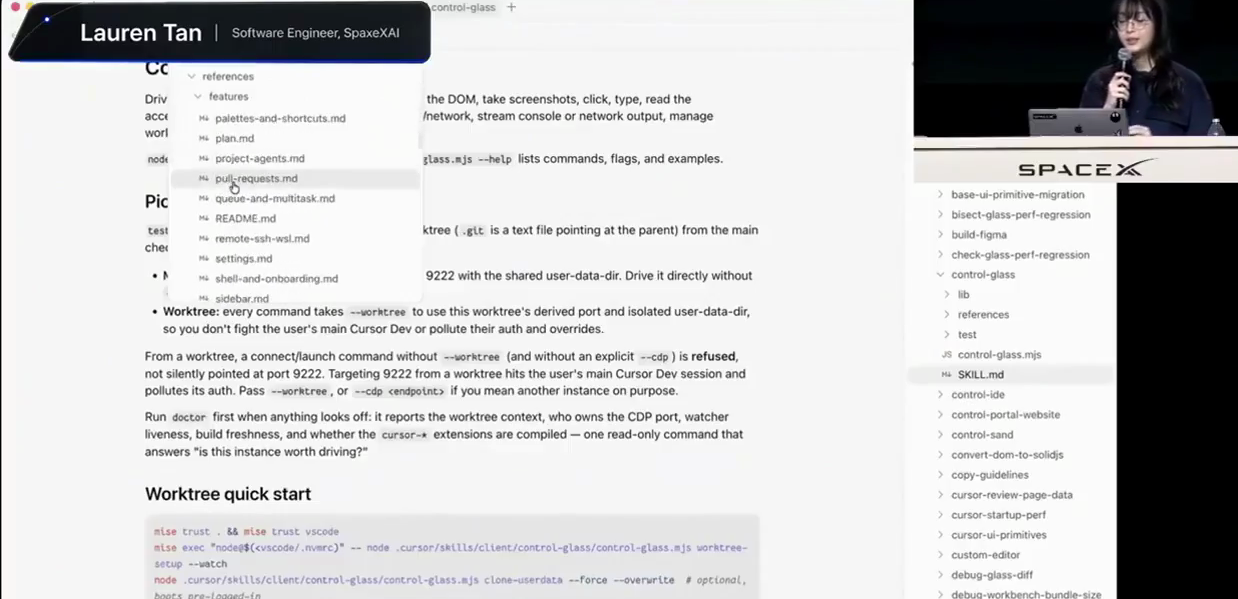
\includegraphics[width=0.92\textwidth]{figures/fig_08_feature_map_files.png}
  \caption{\texttt{control-glass/references/features/} 目录下的模块化功能特性地图文件列表：按产品功能面拆分为 \texttt{palettes-and-shortcuts.md}、\texttt{plan.md}、\texttt{project-agents.md}、\texttt{pull-requests.md}、\texttt{queue-and-multitask.md}、\texttt{sidebar.md} 等独立文档\vtag}
\end{figure}
\srcnote{00:10:00--00:10:15}

如图 8 和图 9 所示，\texttt{Glass feature map} 的核心设计哲学写在总览文件 \texttt{README.md} 的开篇第一段：
\begin{quote}
  \textit{``This directory maps every user-facing Glass feature from the user's point of view: what it is, how to get to it, how to use it, and how to drive it over CDP. One file per feature, plus \texttt{cross-cutting-flows.md} for journeys that span features. Read the relevant file before driving or reproducing that surface. \textbf{These files teach how to use a feature, not how it is built. Read the code for internals, which change faster than any doc.}''}
\end{quote}

这句话道破了工程文档维护的真谛：\textbf{永远不要在验证文档里写内部代码是怎么实现的（因为内部实现每天都在变，写了就会迅速腐化过期），而只从用户视角（User POV）写清楚“这个功能是什么、怎么进到这个界面、怎么操作它、以及怎么通过 CDP 驱动它”！}

\begin{figure}[H]
  \centering
  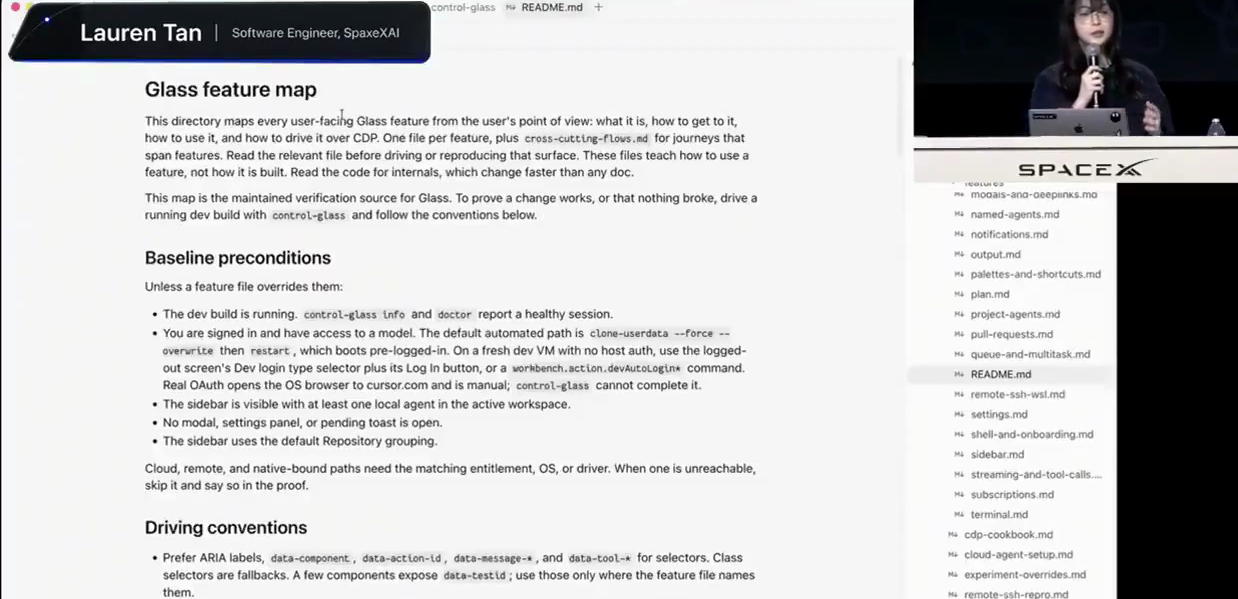
\includegraphics[width=0.92\textwidth]{figures/fig_09_baseline_preconditions.png}
  \caption{\texttt{Glass feature map}（\texttt{README.md}）定义的基线前提条件（\texttt{Baseline preconditions}）：确保智能体在健康、已登录、无遮挡弹窗且处于默认分组的干净状态下开始测试\vtag}
\end{figure}
\srcnote{00:10:30--00:10:45}

在图 9 中，\texttt{Baseline preconditions} 为所有功能测试规定了统一的起跑线：
\begin{enumerate}
  \item 开发构建正在运行，且 \texttt{control-glass info} 与 \texttt{doctor} 均报告健康会话；
  \item 已完成登录且具备模型访问权限（本地默认通过 \texttt{clone-userdata --force --overwrite} 后 \texttt{restart} 启动；在无宿主机凭证的全新云端开发 VM 上，则使用未登录界面的 Dev 登录类型选择器加 \texttt{Log In} 按钮，或触发 \texttt{workbench.action.devAutoLogin*} 命令）；
  \item 左侧边栏可见，且当前活跃工作区中至少存在 1 个本地智能体（Local Agent）；
  \item 当前没有任何模态框（Modal）、设置面板或未关闭的气泡提示（Toast）遮挡界面；
  \item 左侧边栏处于默认的按仓库分组（Repository grouping）状态。
\end{enumerate}

\begin{figure}[H]
  \centering
  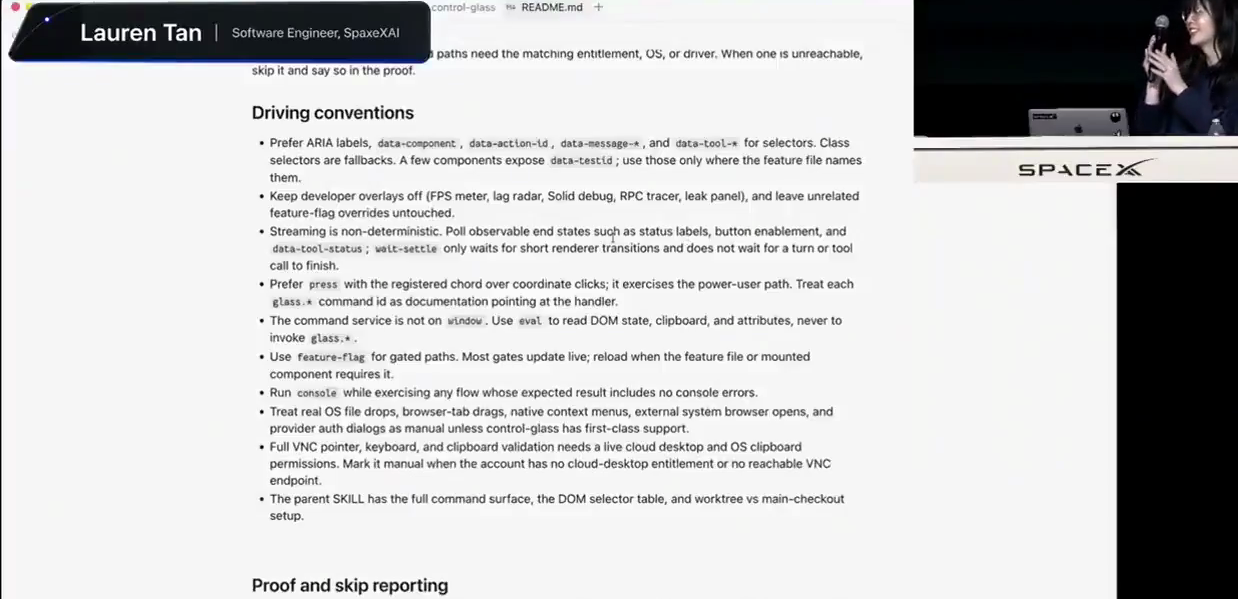
\includegraphics[width=0.92\textwidth]{figures/fig_10_driving_conventions.png}
  \caption{\texttt{Glass feature map} 的驱动约定（\texttt{Driving conventions}）与验证证明报告规范（\texttt{Proof and skip reporting}）\vtag}
\end{figure}
\srcnote{00:11:30--00:11:45}

更进一步，图 10 中的 \textbf{\texttt{Driving conventions}} 为智能体制定了极具实操性的 UI 自动化军规，防止智能体写出脆弱或虚假的验证脚本：
\begin{itemize}
  \item \textbf{选择器优先级铁律}：优先使用 ARIA 标签（\texttt{aria-label}）、\texttt{data-component}、\texttt{data-action-id}、\texttt{data-message-*} 与 \texttt{data-tool-*} 作为选择器；普通 CSS 类名选择器仅作为最后兜底，且仅在特性文档明确点名时才允许使用 \texttt{data-testid}。
  \item \textbf{保持开发者浮层关闭}：测试期间保持 FPS 帧率表（FPS meter）、延迟雷达（Lag radar）、Solid 调试器、RPC 追踪器与内存泄漏面板处于关闭状态，且不得触碰无关的实验特性开关（Feature-flag overrides）。
  \item \textbf{非确定性流式输出的状态轮询}：大模型流式回复（Streaming）的时间是非确定性的，智能体严禁仅靠 \texttt{wait-settle}（它只等待极短的渲染过渡），而必须轮询可观测的终态标志，例如状态标签文本、按钮可用状态（Button enablement）以及 \texttt{data-tool-status}。
  \item \textbf{禁止通过 \texttt{eval} 作弊绕过 UI}：命令服务并未挂载在全局 \texttt{window} 上；智能体只能用 \texttt{eval} 读取 DOM 状态或剪贴板，\textbf{严禁在 \texttt{eval} 里直接调用 \texttt{glass.*} 内部命令}来假装完成了 UI 点击，而必须用 \texttt{press} 触发快捷键或真实点击 DOM 元素，真正走通用户的交互路径！
\end{itemize}

\begin{figure}[H]
  \centering
  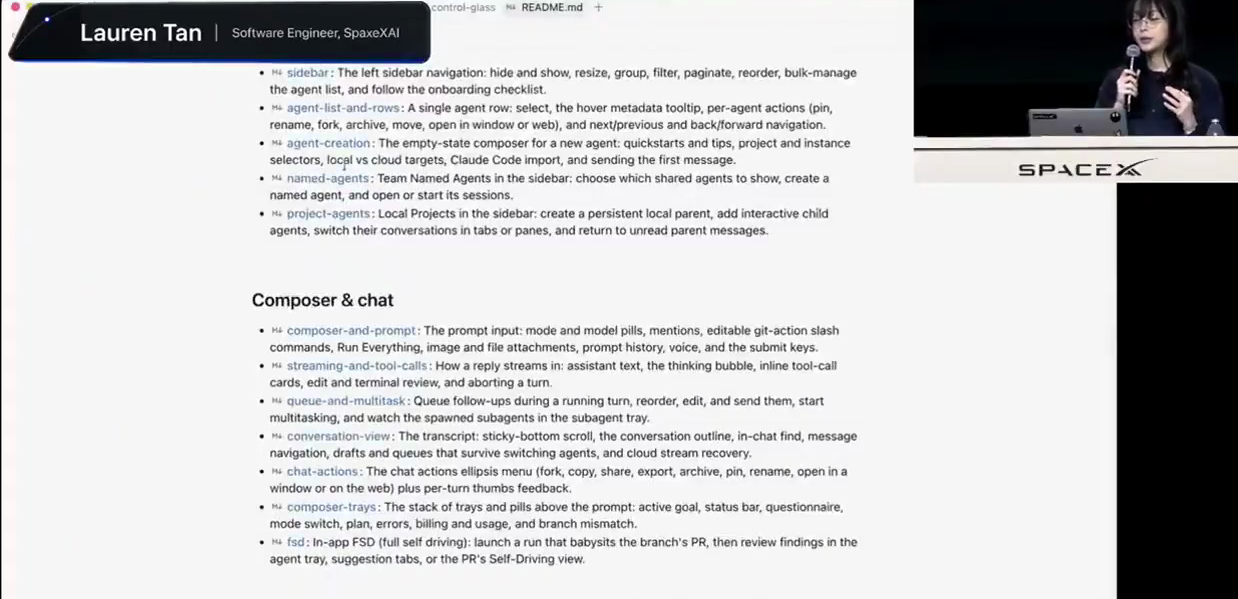
\includegraphics[width=0.92\textwidth]{figures/fig_11_composer_chat_map.png}
  \caption{\texttt{README.md} 中对侧边栏与 \texttt{Composer \& chat} 模块的功能导航索引（涵盖 \texttt{composer-and-prompt}、\texttt{streaming-and-tool-calls}、\texttt{queue-and-multitask}、\texttt{conversation-view}、\texttt{fsd} 全自动驾驶模式等）\vtag}
\end{figure}
\srcnote{00:12:30--00:12:45}

\begin{figure}[H]
  \centering
  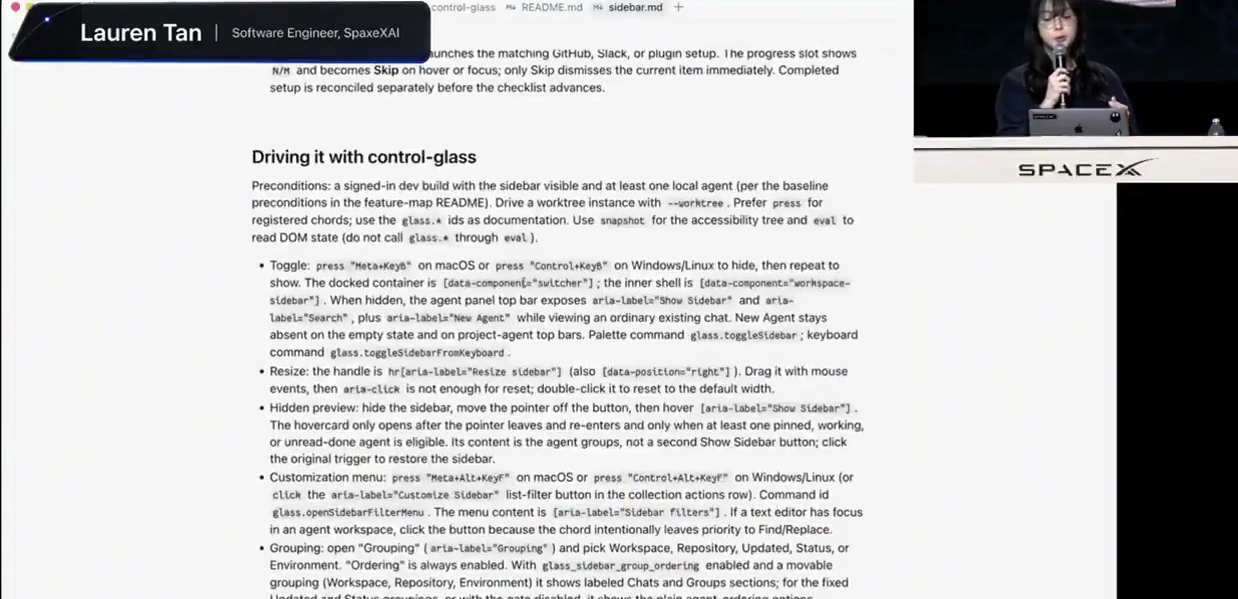
\includegraphics[width=0.92\textwidth]{figures/fig_12_sidebar_driving_recipe.png}
  \caption{\texttt{sidebar.md} 中的 \texttt{Driving it with control-glass} 实操手册：精确定义侧边栏隐藏/展开（\texttt{Toggle}）、拖拽调整宽度（\texttt{Resize}）、悬停预览（\texttt{Hidden preview}）、过滤菜单（\texttt{Customization menu}）与分组排序（\texttt{Grouping}）的每一步 DOM 选择器与快捷键\vtag}
\end{figure}
\srcnote{00:12:45--00:13:00}

当智能体点进任意一个具体特性文件（如图 11 的索引与图 12 的 \texttt{sidebar.md}）时，它就像拿到了一份详尽的“宜家说明书”：
\begin{itemize}
  \item 要测试\textbf{侧边栏折叠与展开（Toggle）}：在 macOS 上调用 \texttt{press "Meta+KeyB"}（Windows/Linux 为 \texttt{Control+KeyB}）；停靠容器选择器为 \texttt{[data-component="switcher"]}，内部壳容器为 \texttt{[data-component="workspace-sidebar"]}；隐藏后顶部栏会暴露出 \texttt{aria-label="Show Sidebar"} 与 \texttt{aria-label="Search"}。
  \item 要测试\textbf{侧边栏拖拽缩放与双击重置（Resize）}：拖拽句柄为 \texttt{hr[aria-label="Resize sidebar"]}（同时带有 \texttt{[data-position="right"]}），注意单独调用 \texttt{aria-click} 不足以重置宽度，必须执行鼠标双击（Double-click）才能恢复默认宽度。
\end{itemize}

\begin{practicebox}{工程落地指南：如何为你自己的项目一键生成并维护 Feature Map？}
很多读者会问：“这样一份详尽的 \texttt{feature-map.md} 写起来岂不是要花好几天？”
Lauren 给出的答案是：\textbf{这份地图本身就是让智能体自动探索代码库并启动真实应用编写出来的！}她已经将这套构建与维护工作流打包进了她的开源插件库 \textbf{\texttt{pstack}}（Potato Stack）中，包含两个开箱即用的技能：
\begin{enumerate}
  \item \texttt{create-verification}：引导智能体扫描你的前端/客户端路由、组件树与快捷键注册表，结合实际拉起应用进行探索，从零生成按用户视角组织的 \texttt{feature-map} 目录；
  \item \texttt{maintain-verification}：当产品新增或修改了 UI 交互后，自动同步更新对应的特性地图文件，确保验证地图永远与最新主干保持一致。
\end{enumerate}
\end{practicebox}

\subsection{本章小结}

本章深入拆解了建立智能体信任的第一支柱——闭环验证（Verification）。通过构建基于 Playwright CDP 的 \texttt{control-glass} 技能，配合 Git Worktree 端口与用户数据隔离（\texttt{Pick a flow} + \texttt{clone-userdata}），十几个并行智能体可以在各自独立的客户端沙盒中免登录启动并采集性能指标。而从用户视角编写的 \texttt{Glass feature map} 则彻底解决了智能体“不知如何导航到目标 UI 状态”的痛点，使端到端复现与回归验证完全脱离了人肉干预。

\clearpage
% ============================================================================
\section{第二支柱：高质量工程技能库 \texttt{pstack} 与技能单元测试（Skill Evals）}
% ============================================================================

\subsection{\texttt{pstack}（Potato Stack）的命名渊源与潜空间引导哲学（13:30--16:00）}

有了闭环验证工具之后，如何让智能体在面对复杂工程问题时，不再像初级实习生那样盲目试错，而是像资深软件工程师一样思考和行动？这就引出了第二大支柱——\textbf{高质量工程技能库（High-Quality Skills）}。

\begin{figure}[H]
  \centering
  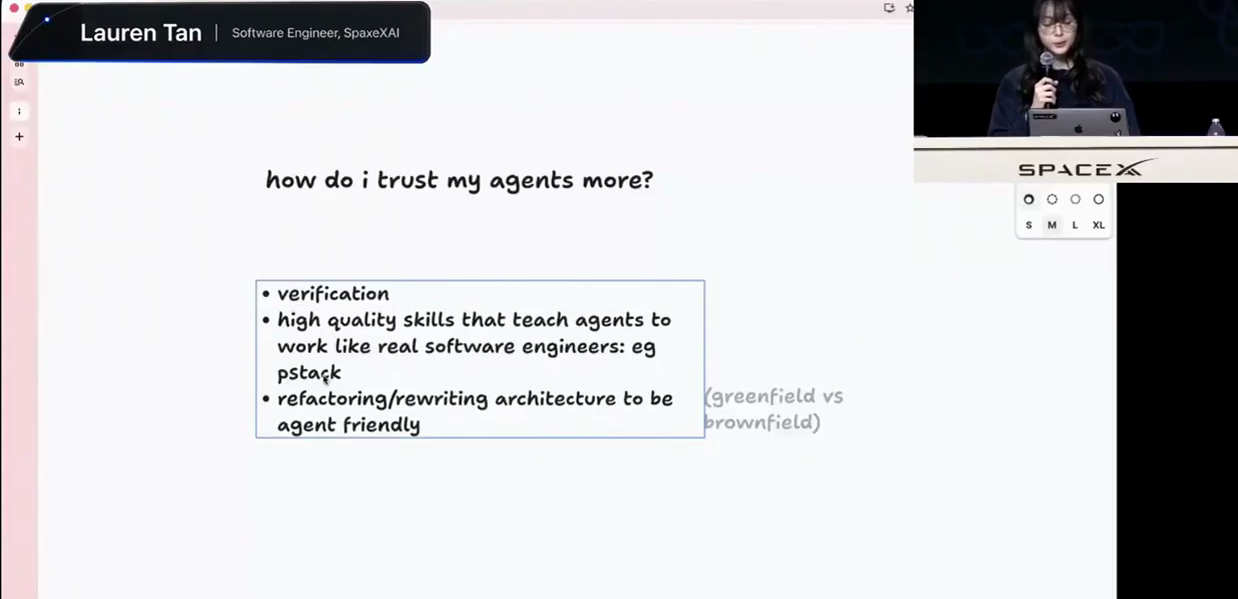
\includegraphics[width=0.88\textwidth]{figures/fig_13_pstack_skills.png}
  \caption{建立智能体信任的第二支柱：教会智能体像真正的软件工程师一样工作的高质量技能库（以开源项目 \texttt{pstack} 为代表）\vtag}
\end{figure}
\srcnote{00:13:30--00:13:45}

Lauren 将她日常沉淀的通用软件工程技能开源在了她的个人项目 \textbf{\texttt{pstack}}（全称 \textbf{Potato Stack}）中。在演讲中，她幽默地解释了这个名字的来历：
\begin{itemize}
  \item 她的网络 ID 叫 \texttt{poteto}（土豆），而 Y Combinator 总裁 Garry Tan 此前开源了一个非常出名的智能体技能栈叫 \texttt{GStack}；
  \item 因为她和 Garry Tan 都姓 Tan（陈），甚至经常有网友在推特上问她“Garry Tan 是不是你叔叔？”（实际上两人毫无亲属关系），于是她干脆将自己的技能栈命名为 \texttt{pstack}（Potato Stack），既是对 \texttt{GStack} 的致敬，也是一次有趣的调侃。
\end{itemize}

从第一性原理来看，\textbf{究竟什么是 Skill（技能）？}
Lauren 指出，Skill 表面上只是一个按需加载的 Markdown 文件（\texttt{SKILL.md}），但从大语言模型的信息论本质来看，\textbf{高质量的 Skill 是一组高密度的先验知识 Token（Prior Tokens），它的作用是在任务开始瞬间，将大模型的激活状态精准推入更高智商、更遵循工程纪律的潜空间区域（Latent Space）}。

\subsection{反模式矫正案例：用 \texttt{/how} 技能根治智能体“不读代码就瞎猜”（16:00--18:00）}

Lauren 分享了她开发每个 Skill 的标准触发机制：\textbf{每当她在日常工作中看到智能体做出令她抓狂的愚蠢行为时，她绝不只在当前会话里骂它一句，而是立刻针对该失败模式提炼出一个通用 Skill。}

最典型的例子就是前面提到的“智能体在修 Bug 时不仔细读代码，连续第 100 次瞎猜自己找到了 Smoking Gun”。为什么智能体会这样？因为通用大模型在预训练与对齐阶段被鼓励“快速给出一个看起来合理的答案”，面对庞大代码库时，它倾向于只看一两个文件名就开始凭直觉编造原因。

为了根治这一顽疾，Lauren 在 \texttt{pstack} 中编写了 \textbf{\texttt{/how}} 技能：
\begin{enumerate}
  \item 当工程师输入 \texttt{/how <问题描述或系统模块>} 时，该技能首先向智能体下达一条硬性禁令：\textbf{严禁猜测（Stop Guessing），严禁在没有源码行号证据的情况下提出任何假设}；
  \item 强制智能体将问题拆解为多条正交的代码追踪线索，并并发派生多个只读子智能体（Sub-agents）深入代码库检索真实的调用栈、状态流转与边界条件；
  \item 要求每个子智能体必须带回精确的文件路径、函数名与代码片段作为呈堂证供，汇总成一份严谨的系统运作机制报告后，才允许进入修复方案设计阶段。
\end{enumerate}

\subsection{谁来测试你的 Skills？——\texttt{eval-playbook} 与防作弊盲测机制（18:00--24:00）}

随着团队和个人编写的 \texttt{SKILL.md} 越来越多、越来越长，一个新的工程难题浮出水面：\textbf{当你修改了某个 Skill 的提示词、或者往里面加了三条新规则时，你怎么知道这个修改真的让智能体变聪明了，而不是引发了退化（Regression）或把原有的好行为搞坏了？}

许多开发者写 Skill 完全靠“玄学感觉（Vibes）”——改两句提示词，跑一次觉得还行就提交了。Lauren 指出，既然我们把构建软件系统的工程纪律带入了智能体时代，那么\textbf{Skills 本身就是代码，必须拥有自己的单元测试（Unit Tests for Skills）——即技能评测（Skill Evals）！}

\begin{figure}[H]
  \centering
  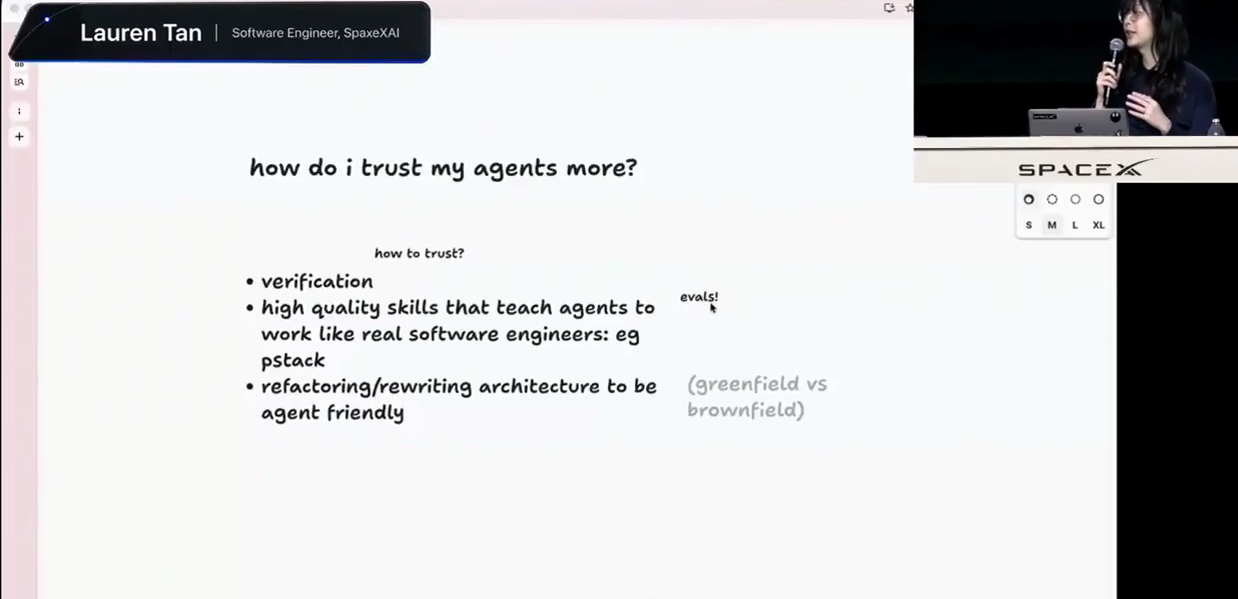
\includegraphics[width=0.88\textwidth]{figures/fig_14_skill_evals.png}
  \caption{第二支柱的闭环保障：为工程技能建立单元测试体系（\texttt{evals!}），通过自动化评测与爬山循环消除提示词玄学\vtag}
\end{figure}
\srcnote{00:18:30--00:18:45}

为此，Lauren 在 \texttt{pstack} 的 \texttt{potato-mode} 插件下专门开源了一个名为 \textbf{\texttt{eval-playbook}} 的元技能（Meta-skill，即“用来评测和优化其他技能的技能”）。\texttt{eval-playbook} 的运作架构极为精妙，包含四个核心环节：

\begin{enumerate}
  \item \textbf{协调器制定正交评分量表（Coordinator \& Rubric Generation）}：
  主协调器智能体（Coordinator Agent）首先读取待测的 \texttt{SKILL.md}，自动分析该技能试图约束的关键工程行为，生成一组具有挑战性的合成测试场景（Test Scenarios）以及一套定量的 10 分制评分量表（Rubric）。
  \item \textbf{防评测察觉的伪装目录盲测（Anti-Sandbagging / Eval-Awareness Defense）}：
  在并发拉起被测子智能体（Subject Sub-agents）执行任务时，协调器会特意为每个子智能体创建一个\textbf{经过伪装命名的真实风格临时工作目录}（例如看起来像真实业务模块的目录名，而不是 \texttt{/tmp/skill-eval-test-1/}），并且在系统提示词中完全隐去任何“测试”“评测”字样。
  \item \textbf{多模型矩阵与异构裁判交叉打分（Cross-Model Judge Matrix）}：
  由于 Cursor 原生支持调用多家主流前沿大模型，\texttt{eval-playbook} 可以在不同基底模型构成的矩阵上并发运行同一套测试，并指派\textbf{异构模型的裁判智能体（Judge Agents）}对照评分量表对被测智能体的轨迹（Trajectory）和产出物进行盲审打分，从而彻底消除单一模型“自己给自己打高分”的自评偏见（Self-Preference Bias）。
  \item \textbf{基于 \texttt{/loop} 的自动爬山优化（Hill-Climbing to 10/10）}：
  结合她编写的 \texttt{/loop} 循环执行技能，智能体可以根据裁判扣分的具体原因，自动微调 \texttt{SKILL.md} 的表述结构，然后重新运行整套盲测，如此迭代爬山（Hill-climb），直到该技能在所有测试场景与模型矩阵上稳定拿到 \textbf{10/10 满分}！
\end{enumerate}

\begin{warningbox}{工程陷阱与警示：为什么要严防智能体“察觉自己正在被评测（Eval Awareness）”？}
Lauren 在演讲中特别强调了一个前沿大模型评测领域的共性现象：现代前沿编码模型具有极强的环境感知能力（Situational / Eval Awareness）。如果被测子智能体从文件夹路径（如 \texttt{eval\_workspace}）或提示词痕迹中察觉到“我现在正处于一场单元测试或能力评测中”，它的行为分布会发生显著偏移——有时会表现得过度讨好教条，有时甚至会出现投机取巧（Sandbagging / Gaming the Eval）的行为，导致评测得出的高分在真实生产环境中完全失真。因此，\textbf{目录伪装与盲测隔离}是保证 Skill Eval 真实有效的关键设计。
\end{warningbox}

我们可以将 \texttt{eval-playbook} 的跨模型爬山优化过程形式化为一个离散提示词空间 $\mathcal{S}$ 上的黑盒优化问题。设待优化的技能文档为 $s \in \mathcal{S}$，测试任务集为 $\mathcal{X} = \{x_1, \dots, x_K\}$，被测执行模型集合为 $\mathcal{M}_{\text{actor}}$，异构裁判模型集合为 $\mathcal{M}_{\text{judge}}$，评分量表函数为 $R(\tau, x) \in [0, 10]$（其中 $\tau$ 为智能体在伪装环境 $\mathcal{E}_{\text{camouflage}}(x)$ 中生成的完整工具调用与代码修改轨迹）。则第 $t$ 轮迭代的技能综合得分 $J(s^{(t)})$ 与更新规则为：
\begin{equation}
  J\bigl(s^{(t)}\bigr) \;=\; \frac{1}{|\mathcal{M}_{\text{actor}}|\cdot|\mathcal{M}_{\text{judge}}|\cdot K} \sum_{m \in \mathcal{M}_{\text{actor}}} \sum_{j \in \mathcal{M}_{\text{judge}}} \sum_{k=1}^{K} R_{j}\!\left(\tau_{m}\bigl(s^{(t)}, \mathcal{E}_{\text{camouflage}}(x_k)\bigr),\; x_k\right)
\end{equation}
在 \texttt{/loop} 循环驱动下，元优化器根据低分轨迹的诊断反馈 $\nabla_{\text{critique}} J(s^{(t)})$ 生成候选修订版 $s^{(t+1)}$，仅当 $J(s^{(t+1)}) > J(s^{(t)})$ 且无单项退化时接受更新，直至收敛至目标阈值 $J(s^*) = 10$。

\subsection{本章小结}

本章探讨了建立智能体信任的第二支柱——高质量工程技能库 \texttt{pstack} 及其评测体系。通过将资深工程师的排障纪律（如强制停止盲目猜测、并发检索代码证据的 \texttt{/how} 技能）编码为高密度先验 Token，智能体得以在更高智商的潜空间中运作；而借助 \texttt{eval-playbook} 的伪装目录盲测、跨模型交叉裁判与 \texttt{/loop} 自动爬山算法（式 (2)），技能文档本身的演进也实现了定量化、工程化的质量保障。

\clearpage
% ============================================================================
\section{米其林三星厨房与云端智能体工厂：自动值班机器人 \texttt{Benny}}
% ============================================================================

\subsection{主厨隐喻：构建你的米其林厨房与软件工厂（24:00--25:15）}

当闭环验证（第一支柱）与高质量工程技能（第二支柱）结合在一起时，软件工程师的日常工作形态会发生怎样的质变？Lauren 在画布上写下了一行极具画面感的标题：\textbf{\texttt{building your michelin kitchen / software factory}}（建造你的米其林三星厨房 / 软件工厂，随后她把略显冰冷的 \texttt{software factory} 划掉，保留了更有温度与品味追求的 \texttt{michelin kitchen}）。

\begin{figure}[H]
  \centering
  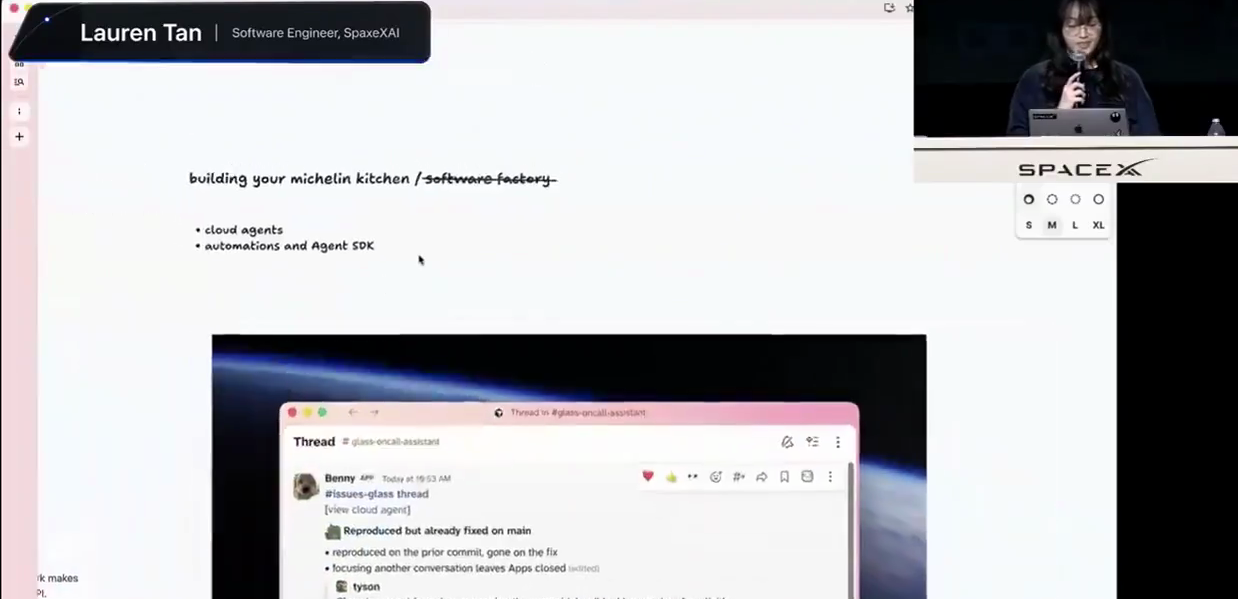
\includegraphics[width=0.88\textwidth]{figures/fig_15_michelin_kitchen.png}
  \caption{米其林厨房隐喻：利用云端智能体（\texttt{cloud agents}）、自动化触发器与 \texttt{Agent SDK} 构建高品味的软件工程厨房\vtag}
\end{figure}
\srcnote{00:24:45--00:25:00}

在一间米其林三星餐厅的后厨里，行政总厨（Head Chef）绝不会一个人从洗菜、切肉、熬汤一直干到把每一盘菜端上桌。相反，总厨的核心职责是：
\begin{enumerate}
  \item \textbf{设计菜单与出品标准（Architecture \& Taste）}：决定餐厅供应什么菜品、确立不可妥协的风味与摆盘标准；
  \item \textbf{规划厨房动线与标准作业程序（Skills \& Verification）}：为副厨（Sous Chefs）和各个档口厨师（Line Cooks——对应负责不同子任务的专业智能体）制定清晰的烹饪配方与出品自检流程；
  \item \textbf{在出菜口进行最终品控（Final Pass Inspection）}：当各档口智能体按标准完成烹制与自检后，总厨只需在出菜口做极快速的最终巡检。
\end{enumerate}

\subsection{从本地观测走向云端规模化：云端复现智能体 \texttt{Benny}（25:15--28:50）}

如何把本地调教好的这套“米其林厨房动线”扩展到服务整个工程团队？Lauren 给出了非常清晰的演进路径：\textbf{从本地（Local）起步构建信任，向云端虚拟机（Cloud Agent VMs）规模化扩张}。
\begin{itemize}
  \item \textbf{为什么必须从本地起步？}因为当你刚开始编写一个新的验证技能（如 \texttt{control-glass}）时，你需要亲眼看着智能体是怎么打开窗口、怎么点歪按钮、怎么卡在某个弹窗上的。本地可视化观测能让你以最快速度修补技能漏洞、建立初始信任。
  \item \textbf{为什么要推向云端？}一旦你在本地完全信任了这套验证闭环，就不应再让它占用你宝贵的笔记本电脑内存和 CPU，而应将其部署到带有完整桌面环境的\textbf{云端智能体虚拟机（Cloud Agents）}中，并通过事件自动化（Automations）与 \texttt{Agent SDK} 全天候触发运行。
\end{itemize}

为了展示云端智能体与 \texttt{control-glass} 结合后的威力，Lauren 晒出了 Cursor 内部 Slack 频道 \texttt{\#glass-oncall-assistant} 中的一张真实工作截图——由团队同事基于她编写的 \texttt{control-glass} 技能搭建的云端值班复现智能体 \textbf{\texttt{Benny}}（头像是一只可爱的狗狗）：

\begin{figure}[H]
  \centering
  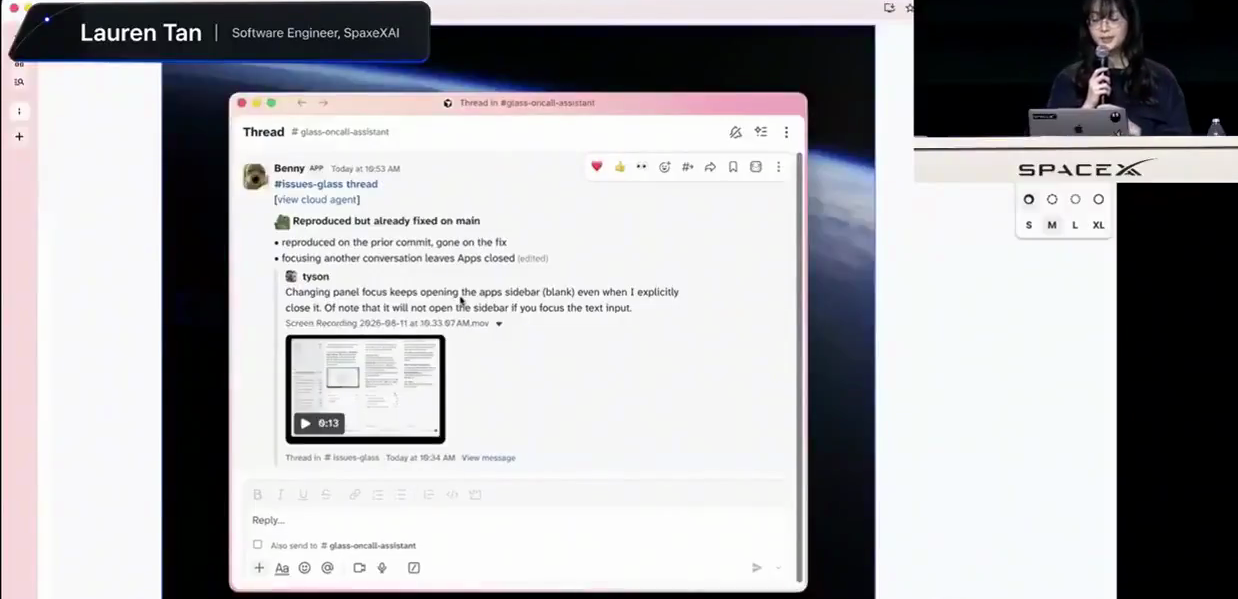
\includegraphics[width=0.90\textwidth]{figures/fig_16_benny_cloud_agent.png}
  \caption{云端值班智能体 \textbf{\texttt{Benny}}（\texttt{\#glass-oncall-assistant}）自动监听 \texttt{\#issues-glass} 报错频道，解析用户上传的 13 秒录屏并在云端沙盒桌面自动复现，给出 \texttt{Reproduced but already fixed on main} 的精准诊断\vtag}
\end{figure}
\srcnote{00:25:30--00:25:45}

让我们仔细研读图 16 中的真实工程细节：
\begin{enumerate}
  \item \textbf{用户上报 Bug（附 13 秒屏幕录像）}：同事 \texttt{tyson} 在 \texttt{\#issues-glass} 频道报告了一个棘手的 UI 焦点问题：\textit{``Changing panel focus keeps opening the apps sidebar (blank) even when I explicitly close it. Of note that it will not open the sidebar if you focus the text input.''}（切换面板焦点时总是会重新打开空白的 Apps 侧边栏，哪怕我已经显式关掉了它；但聚焦文本输入框时不会触发），并附上了一段 13 秒的屏幕录像（\texttt{Screen Recording 2026-06-11 at 10.33.07 AM.mov}，时长 \texttt{0:13}）。
  \item \textbf{\texttt{Benny} 云端自动接单与多模态理解}：事件触发器监听到 \texttt{\#issues-glass} 的新消息后，自动唤醒云端虚拟机中的智能体 \texttt{Benny}。\texttt{Benny} 首先读取报错文本并解析这 13 秒的视频录屏，理解了用户触发 Bug 的精确操作序列。
  \item \textbf{跨版本二分复现与自动结案}：\texttt{Benny} 查阅 \texttt{Glass feature map}，在云端沙盒桌面中拉起开发版客户端，使用 \texttt{control-glass} 严格按照录屏中的操作切换面板焦点。更令人惊叹的是，\texttt{Benny} 不仅在用户报错对应的旧 Commit 上成功复现了该 Bug，还自动在最新的 \texttt{main} 主干分支上跑了一遍相同的操作流，随即在上午 \texttt{10:53 AM} 自动回复诊断结论：
  \begin{itemize}
    \item 状态标签：\textbf{\texttt{Reproduced but already fixed on main}}（已复现，但在主干分支上已被修复）；
    \item 证据说明 1：\texttt{reproduced on the prior commit, gone on the fix}（在前序 Commit 上稳定复现，在修复提交后已消失）；
    \item 证据说明 2：\texttt{focusing another conversation leaves Apps closed}（切换到另一个会话焦点时，Apps 侧边栏保持关闭状态）。
  \end{itemize}
\end{enumerate}

\begin{importantbox}{核心观点：从个人杠杆到团队乘数效应（Team Multiplier）}
试想一下，如果没有 \texttt{Benny}，当值班工程师看到这条报错消息时，需要停下手头的开发工作，花半小时到一小时去拉代码、切分支、看录屏、手动点界面尝试复现，最后才发现“原来半小时前另一个同事的 PR 已经顺带把它修好了”。而现在，Lauren 为解决个人验证瓶颈编写的 \texttt{control-glass} 与 \texttt{feature-map.md}，被同事无缝复用到云端自动化流水线中，在人类工程师介入之前就已经自动完成了\textbf{“视频理解 $\to$ 旧版复现 $\to$ 主干回归验证 $\to$ 自动结案”}的全套闭环！这就是高质量工程技能带来的团队级乘数效应。
\end{importantbox}

\subsection{本章小结}

本章通过“米其林三星厨房”隐喻阐明了现代软件工程师向“行政总厨”的角色转型，并通过云端值班智能体 \texttt{Benny} 的真实生产案例，展示了如何将本地打磨成熟的 \texttt{control-glass} 验证技能推向云端虚拟机，实现从多模态 Bug 报告解析、跨 Commit 自动复现到主干验证的零人工干预闭环。

\clearpage
% ============================================================================
\section{第三支柱：面向智能体友好的架构重构 \texttt{Dune} 与五层防御金字塔}
% ============================================================================

\subsection{Brownfield 与 Greenfield 的反直觉悖论：何时必须重写架构？（28:50--34:30）}

如果说前两大支柱（闭环验证与高质量技能）解决的是智能体在外部如何操作与思考的问题，那么第三大支柱则直指软件工程最核心的腹地：\textbf{代码库本身的软件架构（Software Architecture）}。

在分享她的架构重构经验前，Lauren 提出了一个极其深刻且反直觉的观察：\textbf{为什么在传统万人规模大厂的存量老代码库（Brownfield）里编码智能体往往表现得中规中矩，反而在从零开始完全由 AI 编写的新项目（Greenfield）里，代码库会在短短几周内迅速腐化成没人能改得动的泥潭？}

\begin{figure}[H]
  \centering
  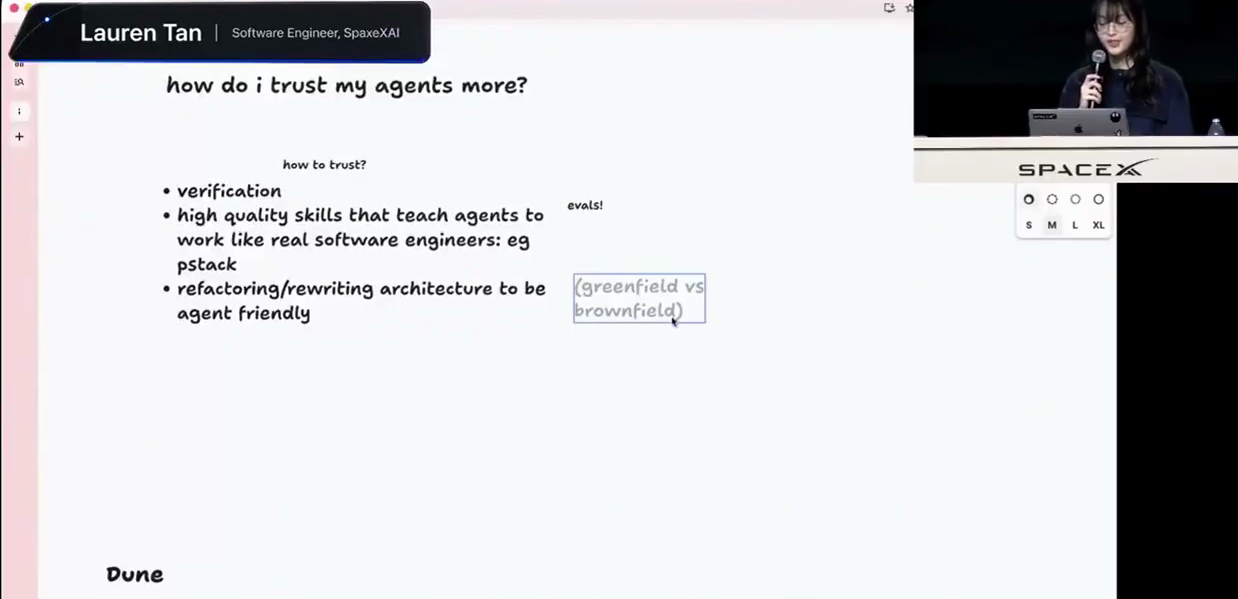
\includegraphics[width=0.88\textwidth]{figures/fig_17_greenfield_vs_brownfield.png}
  \caption{第三支柱核心议题：面向智能体友好的架构重构，以及存量老项目（\texttt{brownfield}）与全新项目（\texttt{greenfield}）的演化差异\vtag}
\end{figure}
\srcnote{00:29:45--00:30:00}

Lauren 结合她在 Meta（拥有数万名工程师与超大型 Monorepo）的工作经历给出了精辟的剖析：
\begin{itemize}
  \item \textbf{成熟 Brownfield 代码库的“防实习生护栏”红利}：
  在 Meta 这样存在了十几年、有上万名人类工程师协同提交的存量代码库中，其实早就充满了大量所谓的“人类烂代码（Human Slop）”。正因为大厂必须假设“每天都有刚入职、不熟悉全局架构的初级工程师或实习生在往仓库里提代码”，大厂的基础设施团队花费了十几年时间，在代码库里建立起了极其严密的\textbf{强类型框架约定、权限隔离、Linter 规则、编译期依赖检查与自动化门禁}——用玩笑话说，大厂的架构本质上是为了“防止实习生一不小心把生产数据库删了”而设计的。当编码智能体进入这种高度结构化、护栏林立的 Brownfield 仓库时，它天然受到既有框架轨道的保护，因此很难把系统彻底搞崩。
  \item \textbf{零人工阅读 Greenfield 项目的“有机架构（Organic Architecture）”灾难}：
  相反，当团队从 0 到 1 快速孵化一个全新的 Greenfield 原型项目——例如他们近期推出的新一代多智能体编排桌面端应用 \textbf{\texttt{Sand}}（音轨中被转播者替换为 \texttt{GrokBot}）——在最初的原型冲刺阶段，为了追求极致的迭代速度，几乎全部代码都是由智能体通过 Vibe Coding 快速生成的，\textbf{没有任何一个人类工程师真正通读过底层代码}！
  在这种毫无护栏的荒野中，智能体每次接到新需求，都会本能地采取当前上下文里最省事的局部捷径。成百上千次局部捷径叠加之后，代码库自发长成了一种失控的\textbf{“有机架构（Organic Architecture）”}：状态散落在几十个文件里互相耦合，同一个功能有三套不同的实现，改东墙必然塌西墙，连最聪明的模型在里面修一个小 Bug 都要原地打转。
\end{itemize}

面对这个失控的 Greenfield 代码库，Lauren 做出了一个果断的工程决策：\textbf{投入 600+ 个原子化 PR，将整个 \texttt{Sand} 应用彻底重写并迁移到她专门为编码智能体量身定制的全新前端/客户端架构——\texttt{Dune}}（取自科幻名著《沙丘》，寓意在狂野的 \texttt{Sand} 之上建立秩序，定位相当于“面向 Electron 桌面应用的 Next.js”）。

\subsection{600+ 个原子化 PR 拆分策略：让 Git 历史成为富上下文源（34:30--37:00）}

为什么重构一个架构要发 \textbf{600+ 个 PR}，而不是像传统架构师那样闭关两周憋出一个包含 40,000 行改动的巨型重写 PR（Mega-PR）？

\begin{figure}[H]
  \centering
  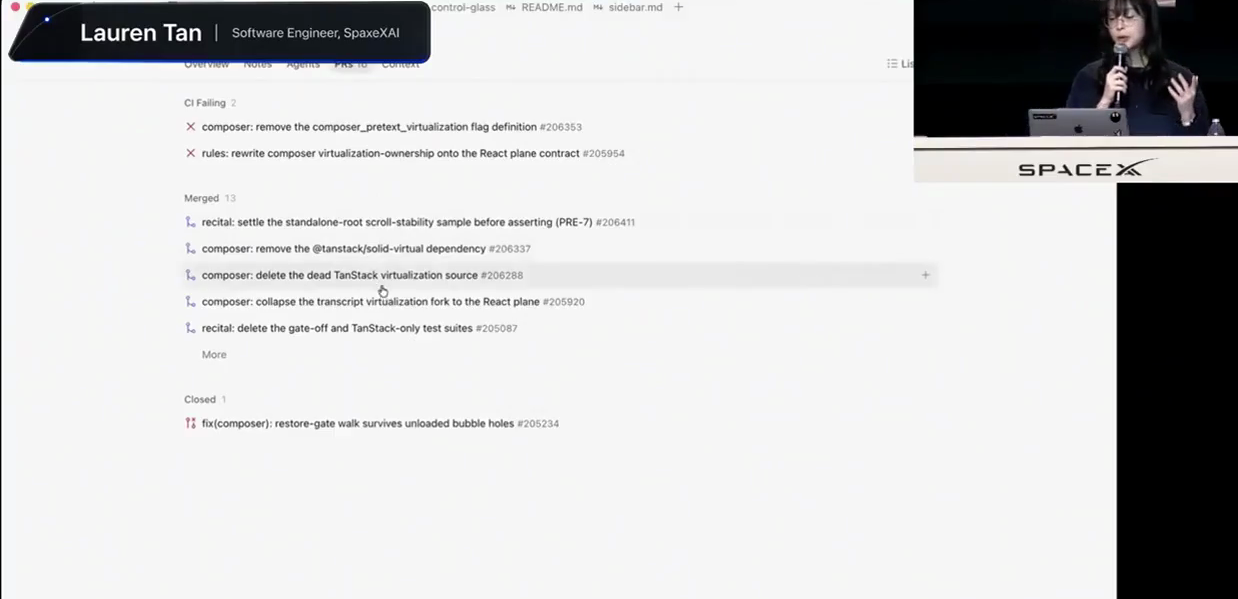
\includegraphics[width=0.92\textwidth]{figures/fig_18_atomic_prs_stack.png}
  \caption{在 Cursor 中将虚拟化引擎重构（从 \texttt{@tanstack/solid-virtual} 迁移至新兴库 \texttt{pretext}）拆解为 16 个高度原子化的 PR 任务栈（已完成合并 \texttt{Merged 13}）\vtag}
\end{figure}
\srcnote{00:36:00--00:36:15}

如图 18 所示，当她准备把客户端聊天转录列表（Transcript）底层的界面虚拟化引擎从原有的 \texttt{@tanstack/solid-virtual} 依赖迁移到新兴的高性能文本与布局虚拟化库 \textbf{\texttt{pretext}} 时，她驱动智能体将其拆解为了 \textbf{16 个环环相扣的原子化小 PR}：
\begin{itemize}
  \item \texttt{recital: settle the standalone-root scroll-stability sample before asserting (PRE-7) \#206411}
  \item \texttt{composer: remove the @tanstack/solid-virtual dependency \#206337}
  \item \texttt{composer: delete the dead TanStack virtualization source \#206288}
  \item \texttt{composer: collapse the transcript virtualization fork to the React plane \#205920}
  \item \texttt{recital: delete the gate-off and TanStack-only test suites \#205087}
\end{itemize}

Lauren 强调，虽然她没有给 PR 设定死板的硬性行数上限（有的 PR 只有 50 行，有的几百行，纯删除死代码的 PR 可能上千行），但她始终强制智能体遵循\textbf{原子化 PR 原则（Atomic PRs）}，原因有三：
\begin{enumerate}
  \item \textbf{任何时刻都可安全回滚（Instant Revertability）}：如果一个 40,000 行的巨型 PR 合并后引发了隐蔽的线上退化，你根本无法回滚（因为其他人的代码已经建立在它之上了）；而 50--200 行的原子 PR 一旦出问题，可以在几秒钟内无痛 Revert。
  \item \textbf{降低智能体与人类的认知负荷}：无论是自动化验证脚本、CI 中的 BugBot 审查，还是人类事后在 \texttt{main} 分支上的巡检，小而专注的 PR 都能确保极高的问题暴露率。
  \item \textbf{把 Git Commit 历史变成智能体最好的上下文源}：当每个 PR 只做一件语义纯粹的事（并附带清晰的提交说明与验证证明）时，未来的智能体在排查问题时通过 \texttt{git log} 或 \texttt{git blame} 就能瞬间读懂架构演进的来龙去脉。
\end{enumerate}

\subsection{\texttt{Dune} 的核心契约（Contract）：顺应智能体的 5 种局部贪婪本能（37:00--40:00）}

究竟什么样的软件架构才叫\textbf{“面向智能体友好（Agent-Friendly Architecture）”}？
在编写 \texttt{Dune} 框架之前，Lauren 没有空谈抽象的设计模式，而是先在架构文档中客观剖析了编码智能体在有限上下文窗口（Context Window）下的\textbf{五种可预测的局部贪婪行为本能}：

\begin{figure}[H]
  \centering
  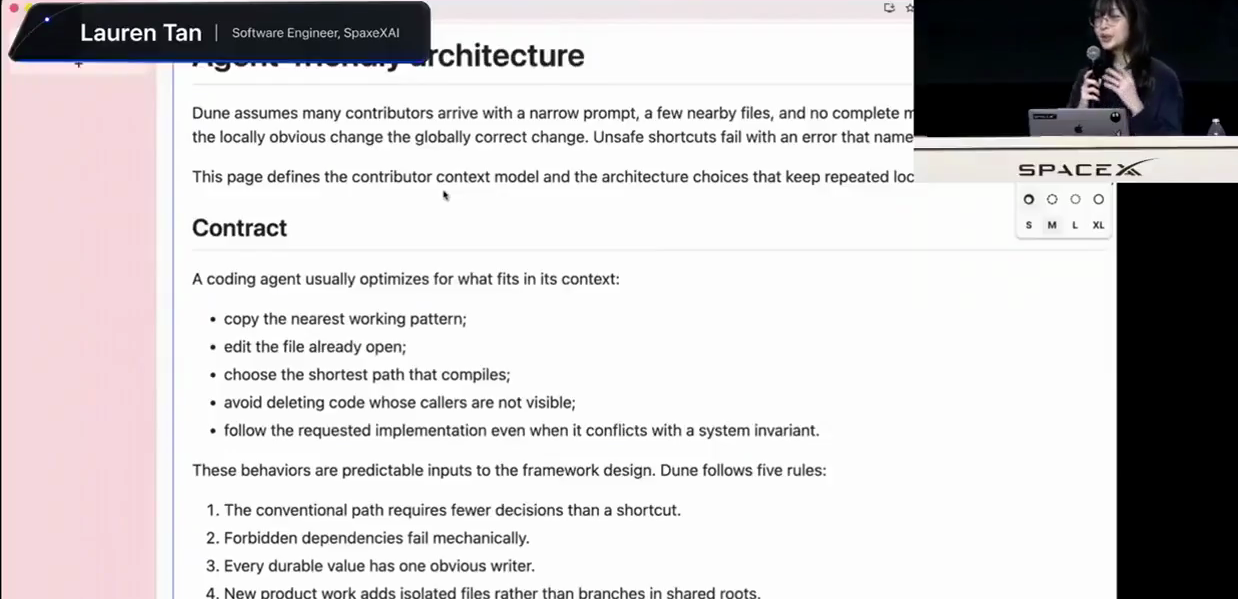
\includegraphics[width=0.92\textwidth]{figures/fig_19_dune_contract.png}
  \caption{\texttt{Dune: Agent-friendly architecture} 核心架构宣言：明确指出编码智能体的 5 种局部上下文优化本能，并据此确立 \texttt{Dune} 的五大架构铁律（Five Rules）\vtag}
\end{figure}
\srcnote{00:38:30--00:38:45}

让我们完整对照图 19 中 \texttt{Dune} 架构文档的原文：
\begin{quote}
  \textit{``Dune assumes many contributors arrive with a narrow prompt, a few nearby files, and no complete model of Sand... Unsafe shortcuts fail with an error that names the supported owner or pattern.}

  \textit{A coding agent usually optimizes for what fits in its context:}
  \begin{itemize}
    \item \textit{\textbf{copy the nearest working pattern;}（复制离它最近的可用代码模式）}
    \item \textit{\textbf{edit the file already open;}（直接修改当前已经打开的文件，而不是去新建或寻找更合适的文件）}
    \item \textit{\textbf{choose the shortest path that compiles;}（选择能通过编译的最短路径）}
    \item \textit{\textbf{avoid deleting code whose callers are not visible;}（只要看不到调用方，就绝不敢删除旧代码，导致死代码无限堆积）}
    \item \textit{\textbf{follow the requested implementation even when it conflicts with a system invariant.}（哪怕用户的表面指令违背了系统底层不变式，也盲目照做）''}
  \end{itemize}
\end{quote}

\begin{importantbox}{\texttt{Dune} 的最高架构哲学：让最短路径成为最正确的路径}
既然编码智能体天性就是“局部贪婪”的——它永远会走阻力最小、决策最少、能最快编译通过的那条路——那么试图靠写文档去说服智能体“不要走捷径”是徒劳的。真正面向智能体友好的架构，必须通过精巧的目录结构与编译期机械约束，实现\textbf{“让智能体本能想走的最短路径，恰好就是全局架构最正确的路径；而任何破坏架构的危险捷径，都会立即触发机械报错（Fail Mechanically），并在报错信息里直接告诉智能体正确的写法是什么”}！
\end{importantbox}

基于这五大行为输入，图 19 底部确立了 \textbf{\texttt{Dune} 的五大架构铁律（Dune Follows Five Rules）}：
\begin{enumerate}
  \item \textbf{\texttt{1. The conventional path requires fewer decisions than a shortcut.}}
  （走符合规范的正道所需的决策步骤，比走野生捷径更少。）
  \item \textbf{\texttt{2. Forbidden dependencies fail mechanically.}}
  （被禁止的跨模块依赖关系在机械检查下直接编译/CI 报错失败。）
  \item \textbf{\texttt{3. Every durable value has one obvious writer.}}
  （每一个持久化状态值都只有唯一且显而易见的写入者，杜绝多处散乱修改状态。）
  \item \textbf{\texttt{4. New product work adds isolated files rather than branches in shared roots.}}
  （开发新产品功能应当体现为新增独立隔离的文件，而不是在全局共享的根文件里不断堆砌 \texttt{if/else} 或 \texttt{switch} 分支。）
  \item \textbf{\texttt{5. Exceptions are narrow, explicit, and reviewed as architecture changes.}}
  （任何破例情况都必须极其狭窄、显式声明，并作为架构级变更接受严苛评审。）
\end{enumerate}

\subsection{激进的静态门禁实践：封杀 \texttt{useEffect}、封杀代码注释与死守 16ms 帧预算（40:00--42:00）}

为了让上述五大铁律具备真正不可逾越的牙齿（Teeth），Lauren 在 \texttt{Dune} 的 CI 与 Linter 中配置了一系列令传统程序员闻所未闻、但在智能体时代却无比高效的硬性静态门禁：

\subsubsection{门禁一：在 CI 中全面封杀 React \texttt{useEffect}}
凡是写过大型 React 应用的工程师都知道，\texttt{useEffect} 是引发无限重渲染循环、陈旧闭包（Stale Closures）、竞态条件与多处状态同步灾难的最大“脚枪（Footgun）”。而编码智能体尤其喜欢滥用 \texttt{useEffect}——每当它发现两个状态对不上时，它的第一反应就是糊一个 \texttt{useEffect} 去监听状态 A 并同步修改状态 B。
在 \texttt{Dune} 架构中，\textbf{\texttt{useEffect} 被静态分析器全面封杀}：只要代码里出现 \texttt{useEffect}，CI 直接变红报错！所有副作用与状态派生必须通过框架受控的数据流原语与显式事件处理器完成。

\subsubsection{门禁二：在 CI 中全面封杀普通代码注释（Banning Code Comments）}
更令人拍案叫绝的是，Lauren 在代码库中\textbf{通过 Linter 一刀切禁止了普通代码注释}！为什么？
因为在她的实际观察中，高达 99\% 的情况下（\texttt{99\% of the time}），编码智能体在代码里留下的注释都是毫无价值的垃圾乃至有害误导！她举了一个让人哭笑不得的真实案例：
\begin{itemize}
  \item 有一次她在某个 PR 的对话框里随口批评了智能体一句：“你在这里不应该这么写”；
  \item 结果智能体在修改代码时，竟然在源码里郑重其事地写下了一行注释：\texttt{// Lauren said you should never do this}（// Lauren 说过你绝对不应该这么做）！
  \item 更可怕的是，当后续其他智能体读到这行注释时，会把针对当时那个特定上下文的临时纠偏，误当成整个代码库神圣不可侵犯的永久全局定律！
\end{itemize}
既然智能体经常把对话上下文里的临时废话写进注释污染代码库，而真正好的代码应当通过清晰的命名与类型自解释（Self-documenting），那么干脆在 CI 中把代码注释彻底禁掉，反而让代码库保持了极致的纯净！

\subsubsection{门禁三：物理隔离 Electron 主进程与渲染进程，死守 16ms（60 FPS）帧预算}
作为一个需要同时展示数十个并发智能体流式输出的 Electron 桌面应用，UI 的丝滑度至关重要。要维持 \textbf{60 FPS} 的流畅帧率，渲染线程（Renderer Thread）处理每一帧的总时间预算 $T_{\text{frame}}$ 严格受限：
\begin{equation}
  T_{\text{frame}} \;=\; T_{\text{react\_render}} + T_{\text{layout\_paint}} + T_{\text{ipc\_io}} \;\le\; \frac{1000\text{ ms}}{60\text{ Hz}} \;\approx\; 16.67\text{ ms} \quad (\text{工程硬预算 } 16\text{ ms})
\end{equation}
在重构前的“有机架构”阶段，智能体在写代码时根本分不清某段逻辑是跑在 Electron 主进程（Node/Host 环境）还是渲染进程（浏览器 UI 线程）里，经常随手在 UI 组件里直接 import 一个包含密集文件 I/O、繁重 JSON 解析或复杂状态计算的服务模块。一旦这些重负载计算混入渲染线程，单帧耗时 $T_{\text{frame}}$ 瞬间突破 16ms，导致界面出现肉眼可见的掉帧与卡顿（Jank）。

在 \texttt{Dune} 中，Lauren 从目录结构与 CI 依赖图（Dependency Graph）层面实施了物理级隔离：
\begin{itemize}
  \item 将源码目录严格切分为 \texttt{electron-main}（主进程/Host）与 \texttt{electron-renderer}（渲染进程/Client）；
  \item 在 CI 中运行静态依赖图分析：任何从 \texttt{electron-renderer} 跨越边界直接导入主进程模块或重型非 UI 依赖的行为，都会在编译期直接报错阻断，从根源上捍卫了 16ms 的渲染帧预算。
\end{itemize}

\subsection{五大公共名词与五层约束防御金字塔（42:00--46:50）}

那么，\texttt{Dune} 是如何把上述五大铁律落到具体目录结构上的？让我们看图 20 展示的架构文档下半部分与手绘金字塔：

\begin{figure}[H]
  \centering
  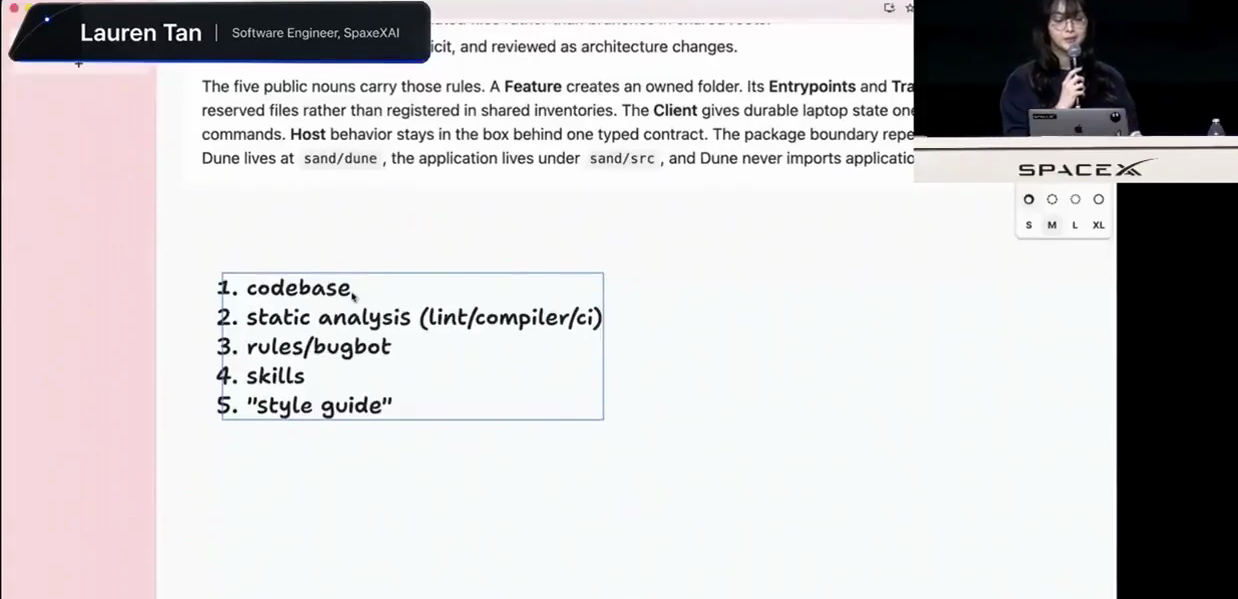
\includegraphics[width=0.92\textwidth]{figures/fig_20_dune_enforcement_layers.png}
  \caption{\texttt{Dune} 架构的五大公共名词（\texttt{Feature}、\texttt{Entrypoints}、\texttt{Transcript cards}、\texttt{Client}、\texttt{Host}）包边界设计，以及从代码库结构到风格指南的五层约束防御金字塔\vtag}
\end{figure}
\srcnote{00:41:45--00:42:00}

如图 20 顶部段落所示，\texttt{Dune} 用\textbf{五大公共名词（Five Public Nouns）}承载了全部架构规则：
\begin{enumerate}
  \item \textbf{\texttt{Feature}（特性自治文件夹）}：每一个产品特性都在 \texttt{sand/src} 下拥有一个完全自治的专属文件夹。得益于极致的\textbf{共置原则（Co-location）}，对于高达 80\% 的日常开发工作（\texttt{And for 80\% of the work}），智能体只需要在同一个文件夹内新增或修改文件，完全不需要跨越目录去修改全局根文件！
  \item \textbf{\texttt{Entrypoints}（入口点）}与 \textbf{3. \texttt{Transcript cards}（转录卡片）}：全部通过特性文件夹内的\textbf{保留文件名（Reserved Files，类似 Next.js 的 \texttt{page.tsx} / \texttt{layout.tsx}）自动发现与挂载}，而不是让智能体去某个全局共享的注册清单（Shared Inventories）里手动加一行 import 和注册分支——这不仅契合了第 4 条铁律，还顺带彻底消除了多个并发智能体同时修改全局注册表引发的 Git 合并冲突（Merge Conflicts）！
  \item \textbf{\texttt{Client}（客户端持久化状态）}：为笔记本本地持久化状态提供受具名 Hook 保护的唯一写入通道（单一明确写入者）。
  \item \textbf{\texttt{Host}（宿主行为契约）}：所有底层宿主操作都被封装在单一强类型契约（Typed Contract）的黑盒背后。此外，框架包本身位于 \texttt{sand/dune}，业务应用位于 \texttt{sand/src}，且 \textbf{\texttt{Dune} 严禁反向导入任何业务应用代码（\texttt{Dune never imports application code}）}。
\end{enumerate}

在演讲的最高潮部分，Lauren 在图 20 下方手绘了\textbf{约束智能体行为的五层防御体系（从硬到软排序）}：
\begin{enumerate}
  \item \textbf{第 1 层（最硬/最强约束）：\texttt{1. codebase}（代码库目录结构与文件共置模式）}
  \item \textbf{第 2 层（机械硬门禁）：\texttt{2. static analysis (lint/compiler/ci)}（静态分析、编译器类型与自定义 Lint/CI 门禁）}
  \item \textbf{第 3 层（自动化软审查）：\texttt{3. rules/bugbot}（Cursor Rules 与 CI 上的 AI 代码审查机器人 BugBot）}
  \item \textbf{第 4 层（工作流操作手册）：\texttt{4. skills}（如 \texttt{pstack} 与 \texttt{control-glass} 等技能文档）}
  \item \textbf{第 5 层（最软/最弱约束）：\texttt{5. "style guide"}（传统的自然语言代码风格指南文档）}
\end{enumerate}

\begin{table}[H]
  \centering
  \caption{编码智能体五层约束防御金字塔（Enforcement Pyramid）对比分析表}
  \small
  \begin{tabular}{c l p{2.6cm} p{3.6cm} p{4.4cm}}
    \toprule
    \textbf{层级} & \textbf{防御层名称} & \textbf{约束性质与硬度} & \textbf{在 \texttt{Dune} / Cursor 中的实例} & \textbf{为什么单靠下层不够？} \\
    \midrule
    L1 & \texttt{codebase} & 物理拓扑引力（最强） & \texttt{Feature} 单目录共置、保留文件名自动发现 & 智能体本能复制最近模式；好目录让正确写法阻力最小 \\
    L2 & \texttt{static analysis} & 编译/CI 机械阻断（硬性） & 禁用 \texttt{useEffect}、禁用注释、进程依赖图隔离 & 违规直接令 CI 变红，确定性拦截，零人工成本 \\
    L3 & \texttt{rules/bugbot} & 自动化 AI 审查（中软） & \texttt{.cursor/rules}、PR 阶段的 BugBot 自动挑错 & 属于概率性软约束，上下文过长时模型仍可能遗忘 \\
    L4 & \texttt{skills} & 按需加载工作流（软性） & \texttt{control-glass}、\texttt{pstack}（\texttt{/how}、\texttt{eval-playbook}） & 擅长引导复杂多步操作流，但不能替代底层编译期类型安全 \\
    L5 & \texttt{"style guide"} & 自然语言文档（最弱） & 写在 Wiki 里的《代码规范指南》 & 智能体极少主动通读，人类靠肉眼在 PR 里抓规范必陷地狱 \\
    \bottomrule
  \end{tabular}
\end{table}

\begin{warningbox}{核心警示：把每一次人工 Code Review 批评都视为架构的失败！}
指着图 20 的五层清单，Lauren 发出了振聋发聩的警告：
许多团队在引入 AI 编码后，试图只靠第 3、4、5 层（写一堆 Cursor Rules、Skills 或风格指南文档）来维持代码质量。但因为第 3、4、5 层本质上都是\textbf{概率性的软约束（Soft Constraints）}，智能体在长上下文中总会遗忘或打折扣。如果缺乏第 1 层（代码库拓扑）和第 2 层（静态分析硬门禁）的兜底，结果必然是两个灾难之一：
\begin{enumerate}
  \item 要么你放任不管，代码库在几个月内彻底沦为无法维护的垃圾场；
  \item 要么你被迫亲自上阵，每天花好几个小时在 PR 里肉眼审查智能体的代码，一遍遍重复写下“这里不要用 \texttt{useEffect}”“那里不要跨进程导入”——\textbf{恭喜你，你把自己困在了“Code Review 地狱”里！}
\end{enumerate}
Lauren 的铁律是：\textbf{每当你在人工 Code Review 中对智能体写下一句修改意见时，你都应该停下来反思——为什么这个问题需要我用肉眼看出来？我能不能把它下沉到第 2 层（写一条自定义 Lint 规则或编译器检查让 CI 直接变红），甚至下沉到第 1 层（修改框架设计，让这类错误在分类学上根本无法被表达出来，就像没有写 \texttt{unsafe} 的 Rust 代码天然不会出现内存安全漏洞一样）？}
\end{warningbox}

我们可以将五层防御体系下系统残余架构缺陷流入主干分支的概率 $P_{\text{escape}}$ 建模为各层拦截率的级联乘积。设智能体原始生成包含某类架构违规的先验概率为 $p_0(G_{\text{codebase}})$（它是第一层代码库拓扑结构 $G_{\text{codebase}}$ 的函数：共置度越高、最近邻模式越干净，$p_0$ 越低），第 $i \in \{2, 3, 4, 5\}$ 层的违规拦截率分别为 $\eta_{\text{static}}, \eta_{\text{bugbot}}, \eta_{\text{skill}}, \eta_{\text{guide}} \in [0, 1]$，则违规逃逸至人工审查阶段的概率为：
\begin{equation}
  P_{\text{escape}} \;=\; p_0(G_{\text{codebase}}) \cdot (1 - \eta_{\text{static}}) \cdot (1 - \eta_{\text{bugbot}}) \cdot (1 - \eta_{\text{skill}}) \cdot (1 - \eta_{\text{guide}})
\end{equation}
由于第 3、4、5 层均为大模型概率性遵循（$\eta_i < 1$），只要 $\eta_{\text{static}} = 0$，$P_{\text{escape}}$ 就始终大于零，随着月提交 PR 数量 $M \to 3000$，逃逸缺陷总数 $M \cdot P_{\text{escape}}$ 必然压垮人类审查者；反之，一旦将规则编码进第 2 层机械静态门禁使 $\eta_{\text{static}} = 1$（或通过第 1 层框架设计使 $p_0 = 0$），则无论并发提交多少千个 PR，该类架构违规的逃逸概率恒为 $P_{\text{escape}} \equiv 0$！

\subsection{本章小结}

本章全面拆解了第三支柱——面向智能体友好的架构重构 \texttt{Dune}。通过剖析成熟 Brownfield 仓库与零人工阅读 Greenfield 项目的反直觉差异，我们理解了为何必须用 600+ 个原子化 PR 重构失控的“有机架构”。\texttt{Dune} 顺应智能体的 5 种局部贪婪本能，以五大铁律和五大公共名词实现了单文件夹改动共置，并通过禁用 \texttt{useEffect}、禁用普通注释、隔离 Electron 主进程与渲染进程（死守 16ms/60FPS 帧预算）等激进 CI 门禁，将软性规范彻底下沉为代码库拓扑与静态分析硬约束（式 (3)--(4)）。

\clearpage
% ============================================================================
\section{炉边问答：Token 成本 ROI、帕累托前沿与全员跨界交付}
% ============================================================================

在演讲的最后 8 分钟里，主持人 Colin 与 Lauren Tan 围绕工程管理者最关心的三个现实问题——\textbf{Token 算力成本的投入产出比（ROI）}、\textbf{模型选择与团队规模}以及\textbf{非工程角色（PM/设计师）的跨界交付}——展开了精彩的深度对话。

\subsection{烧掉海量 Token 重构架构的 ROI 账本：用算力换取组织极简（46:50--49:30）}

主持人 Colin 提出了一个非常犀利的问题：“你在 Cursor 内部几乎拥有无限的 Token 额度，所以你可以花 600 多个 PR、跑无数的子智能体评测去重构 \texttt{Dune} 架构。但对于外部那些需要精打细算控制 AI 预算的创业公司或工程副总裁（VP of Engineering）来说，怎么算这笔经济账？”

Lauren 给出了极具战略高度的回答：\textbf{前期投入 Token 重构强约束架构，本质上是一笔“一次投入、永久降低后续边际推理成本与人力沟通成本”的高杠杆投资}。
\begin{enumerate}
  \item \textbf{让更便宜、更笨的模型也能写出高质量代码}：
  在一个混乱的“有机架构”代码库里，即便你每次都调用最昂贵的顶级超大模型，它也会频频出错；但当你花费前期 Token 将代码库重构为像 \texttt{Dune} 这样“最短路径即正确路径、错误路径机械报错并自带修复提示”的强约束架构后，\textbf{哪怕是价格低廉、参数量小得多的轻量级模型（Dumber / Cheaper Models），也能在严格的轨道内写出完全符合规范的高质量代码！}
  \item \textbf{一个人完成过去一个平台团队数年的工作，避免组织膨胀}：
  在传统软件时代，像 \texttt{Dune} 这样的客户端框架迁移加上全套静态分析门禁，往往需要专门组建一个 5--10 人的前端基础设施/平台团队（Platform Team）干上一整年。而一旦公司人数从几十人膨胀到几百人乃至上万人，随之而来的跨部门协调、会议对齐与管理损耗将呈平方级爆炸（即经典的 Brooks 定律）。现在，借助编码智能体，\textbf{1 名资深工程师花几周的 Token 就能独立完成过去整个平台团队的基建工作}，从而让创业公司能够以百人以内的极简精干团队（Nimble Team）爆发出超越传统万人大厂的工程吞吐量。跟省下的数百万美元人力与管理内耗相比，重构架构烧掉的 Token 费用几乎可以忽略不计。
\end{enumerate}

\subsection{模型智商与成本的帕累托前沿（49:30--51:00）}

紧接着，Colin 与 Lauren 探讨了大模型本身的演进趋势。就在演讲当天，新一代前沿模型刚刚发布（音轨口述为 \texttt{Grok 4.6}，对应原版语境下的 \texttt{Claude 4.6}）。Lauren 指出：
\begin{itemize}
  \item 新一代 4.6 模型在保持与上一代 4.5 模型\textbf{完全相同的单 Token 价格}的前提下，提供了显著跃升的代码推理与工具调用智商，并且由于更少走弯路，在完成相同任务时的实际 Token 消耗反而更高效；
  \item 这意味着模型能力与推理成本的\textbf{帕累托前沿（Pareto Frontier）}正在持续向“更聪明、更便宜、更省 Token”的方向快速推移。当外部的帕累托前沿推进与内部的 \texttt{Dune} 强约束架构相结合时，团队完全可以按任务复杂度动态路由模型，无需在所有常规 CRUD 任务上都盲目烧掉最昂贵的推理算力。
\end{itemize}

\subsection{具名智能体编排与赋能 PM、设计师、GTM 全员直接交付代码（51:00--54:07）}

在访谈的最后，Colin 请 Lauren 介绍了她耗时 600+ 个 PR 重构的这款新产品——\textbf{\texttt{Sand}}（音轨口述为 \texttt{GrokBot}）究竟带来了怎样的新范式。

Lauren 解释道，传统的 AI 编码工具（无论是 IDE 插件还是终端 CLI）在界面与心智模型上仍然是高度面向硬核软件工程师的专业工具，对产品经理（PM）、设计师（Designers）或市场拓展（GTM）人员来说门槛依然很高。而新推出的多智能体编排应用采用了类似 \textbf{iMessage / 即时通讯软件}的亲切交互界面，带来了两大变革：
\begin{enumerate}
  \item \textbf{持久化的具名智能体（Persistent Named Agents）}：
  每个用户都可以在侧边栏里创建并管理多个有名字、有专属记忆和职责的持久智能体。例如：
  \begin{itemize}
    \item 销售与 GTM 团队可以为每一个重点客户账号（Account）专门配置一个具名智能体，持续追踪该客户的所有需求、工单与定制化配置；
    \item Lauren 团队的产品经理专门配置了一个具名智能体，每天早上自动扫描并向 PM 汇报：“Lauren 昨晚睡觉时又往主干合并了哪几十个 PR、上线了什么新功能”，省去了开早会同步进度的时间！
  \end{itemize}
  \item \textbf{强架构护栏赋能非技术角色直接提 PR 修 Bug}：
  更令人兴奋的是，因为 \texttt{Dune} 架构已经在第 1 层（目录共置）和第 2 层（CI 静态分析门禁）建立起了铜墙铁壁般的自动化护栏，再加上 \texttt{control-glass} 的自动端到端验证，\textbf{团队里的设计师和产品经理现在看到界面细节不满意或发现小 Bug 时，不再需要提工单排期等工程师来改，而是直接自己在应用里唤醒智能体修改代码、自动跑通验证并提交 PR，而且一次性就能通过审查合并上线！}
\end{enumerate}

\begin{practicebox}{工程落地指南：面向技术管理者与工程师的行动清单}
如果你想在自己的团队中复刻 Lauren Tan 的“高信任度智能体工程体系”，请按以下优先级逐步落地：
\begin{enumerate}
  \item \textbf{第一步（本周即可落地）}：停止人肉点界面测 AI 代码！参考 \texttt{control-glass} 与开源库 \texttt{pstack} 的 \texttt{create-verification}，用 Playwright/CDP 为你的应用编写自动化驱动脚本，并从用户视角生成一份 \texttt{feature-map.md}，确保支持基于 Git Worktree 的端口与数据隔离。
  \item \textbf{第二步（沉淀与评测技能）}：每当发现智能体重复犯蠢（如不读代码瞎猜），立即编写针对性的 \texttt{SKILL.md}（如 \texttt{/how}），并使用 \texttt{eval-playbook} 在伪装目录中进行盲测与 \texttt{/loop} 爬山优化。
  \item \textbf{第三步（把人工 Review 转化为机械门禁）}：审视你最近两周在 PR 里写下的所有人工审查意见，将它们转化为 ESLint/Biome 自定义规则、模块依赖图边界检查或框架级约束（如封杀高危 API、强制单目录共置与保留文件名自动注册），直至你敢于开启夜间自动合并（Auto-merge）。
\end{enumerate}
\end{practicebox}

\subsection{本章小结}

本章总结了炉边问答的核心洞察：前期消耗 Token 将代码库重构为强约束架构，能够让廉价模型也产出高质量代码，帮助团队维持百人以内的极致精简与敏捷；而结合模型帕累托前沿的推进与 \texttt{Dune} 严密的自动化护栏，不仅工程师能够实现单月千级 PR 的吞吐，连产品经理、设计师与 GTM 团队也能安全、自信地直接向生产代码库交付改动，真正开启了人机协同软件工程的新纪元。

\end{document}
